\section{绪论}
%\pagestyle{plain}
\setcounter{page}{1}%该页页码为第一页
\pagenumbering{arabic}
%\setcounter{page}{1}
%\pagestyle{plain}
\subsection{拓扑绝缘体}
\qquad1980年实验物理学家Kalus von Klitzing在二维电子气中加入高磁场,发现体系的霍尔电阻随着磁场强度改变的时候出现了一些非常平整的平台\upcite{re1}。这种整数化的平台其实是量子效应的一种宏观表现,正是这个发现为人们打开了研究拓扑物态的大门,而Kalus von Klitzing也因此获得了1985年的诺贝尔物理学奖。当均匀的电子气处于强磁场的时候会形成Landua能级,如果体系的费米面恰好处于Landua能级的中间,由能带论可知系统此时处于绝缘状态。但是之后的研究却发现虽然在强磁场下体系内部是绝缘的,但是在边界上却形成了无耗散的导电通道,正是这些通道的存在形成了平台化的霍尔电阻。1982年David J. Thouless,J.Michael Kosterlitz等人(TKNN)对这个量子化的平台给出了完美的解释\upcite{re2}。通过Kubo公式求解体系霍尔电导发现它和一个正数是相关的,也就是说霍尔电导等于$ne^2/h$,这里的正数$n$表示为:
\begin{equation}	
n=\frac{1}{2}\int_{\mathrm{BZ}}d^2k\nabla_k\times i\sum_{l\in\mathrm{bands}}\langle\varphi_l|\nabla_k|\varphi_l\rangle\label{chern_num}
\end{equation}
人们将正数$n$称为第一陈数(Chern Number)。从能带论的角度出发进行考虑,陈数代表的是二维电子气系统的一种拓扑性质,在不闭合体系能隙的时候,连续地改变哈密顿量不会引起它的改变,所以被称为拓扑不变量,这个量仅关联与电子态的拓扑性质。把环境与均匀二维电子气当作一个整体,当电子态从电子气体系中演化到环境的时候,陈数将会由非零变为零,那么在环境与电子气的交界处必须存在着一个能隙为零的界面来过渡,这样才可以实现陈数的变化。霍尔电导与陈数之间的这种深刻联系完美解释了霍尔电导量子化平台的起源,也打开了拓扑物态在物理学领域的应用大门。
\begin{figure}[h]
\centering
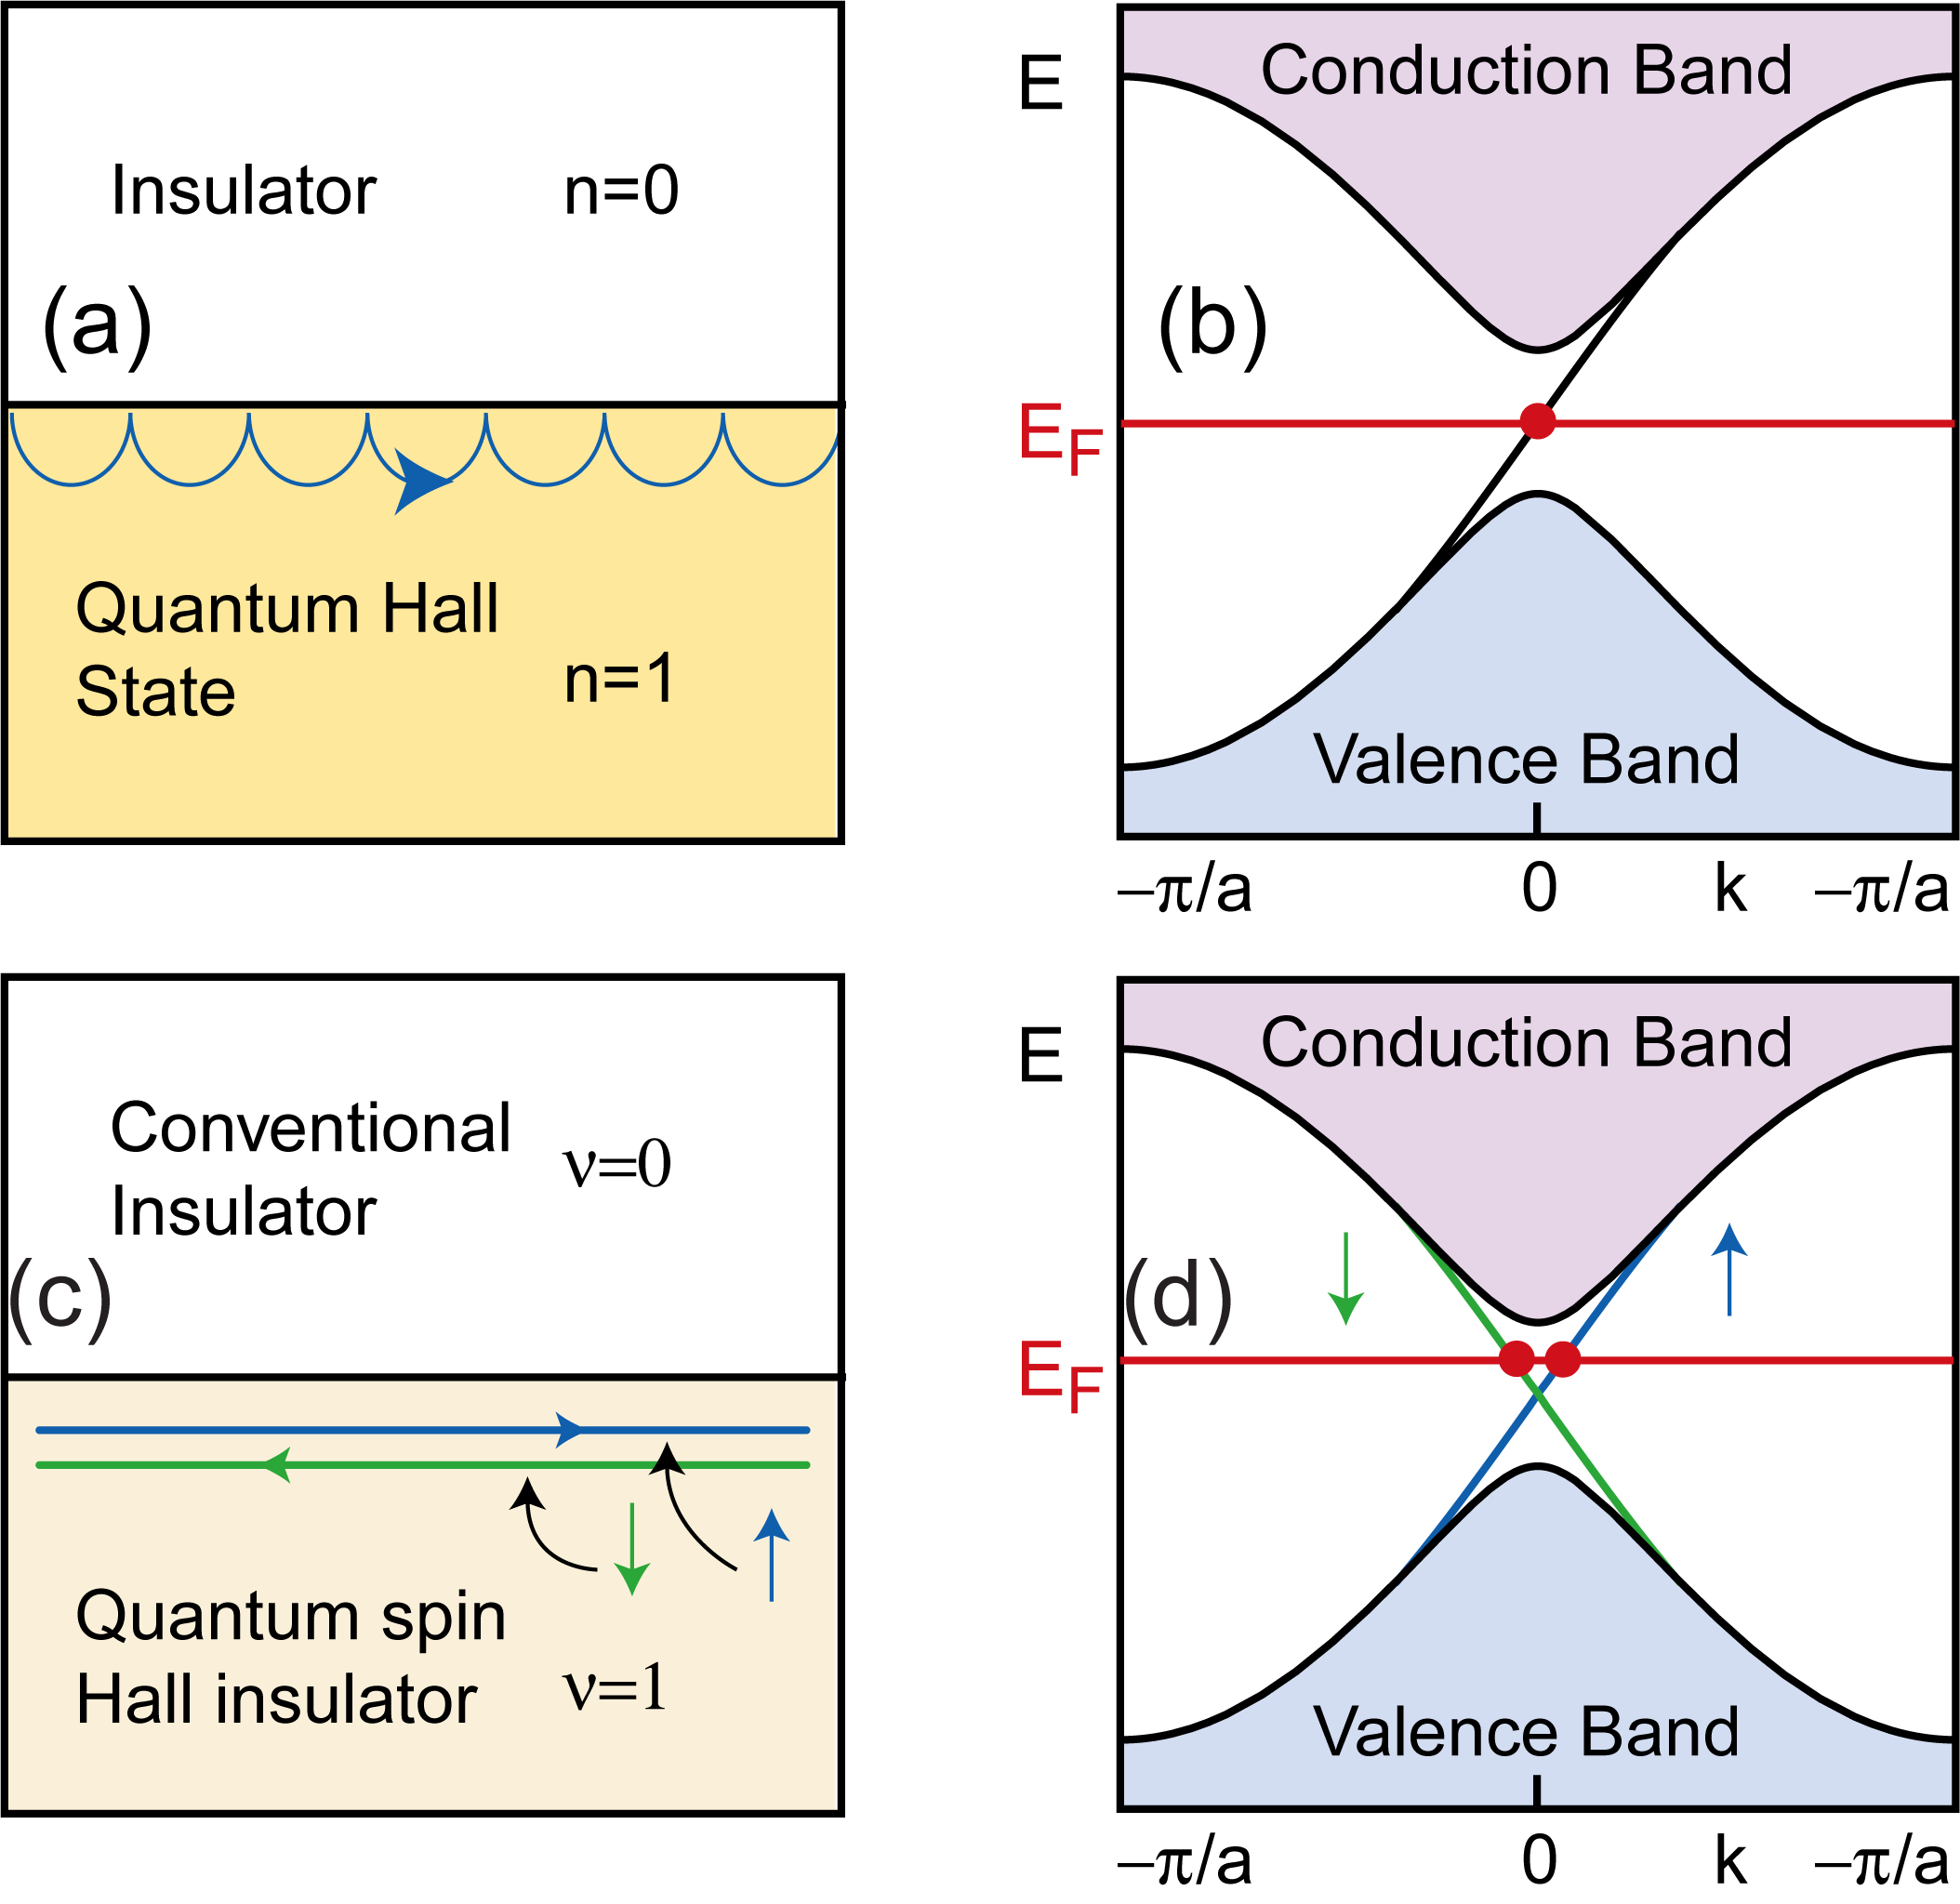
\includegraphics[scale=0.5]{pic/fig1.png}
\caption{(a)整数量子霍尔效应示意图。(b)整数量子霍尔效应能带示意图。(c)整数量子自旋霍尔效应示意图。(d)整数量子自旋霍尔效应能带示意图。}\label{fig1}
\end{figure}
由加磁场产生的整数量子霍尔效应(QHE)以及由晶体自发磁化产生的反常量子霍尔效应(QAHE)都是破坏时间反演对称(TRS)的,但还存在一种满足TRS的量子自旋霍尔效应(QSHE),1988年F.Duncan M.Haldane在六角点阵中通过引入一个净磁通为零的位相,首次在理论上提出了一个不需要宏观磁场就可以实现QSHE,并计算拓扑保护的表面态\upcite{re3}。这种新的量子态可以在存在自旋轨道耦合(SOC)的系统中出现,由于系统满足TRS,所以(\ref{chern_num})中的积分在整个布里渊区(BZ)中为零,也就是陈数为零,这个时候就需要一个新的拓扑不变量来描述QSHE。

\begin{figure}[h]
	\centering
	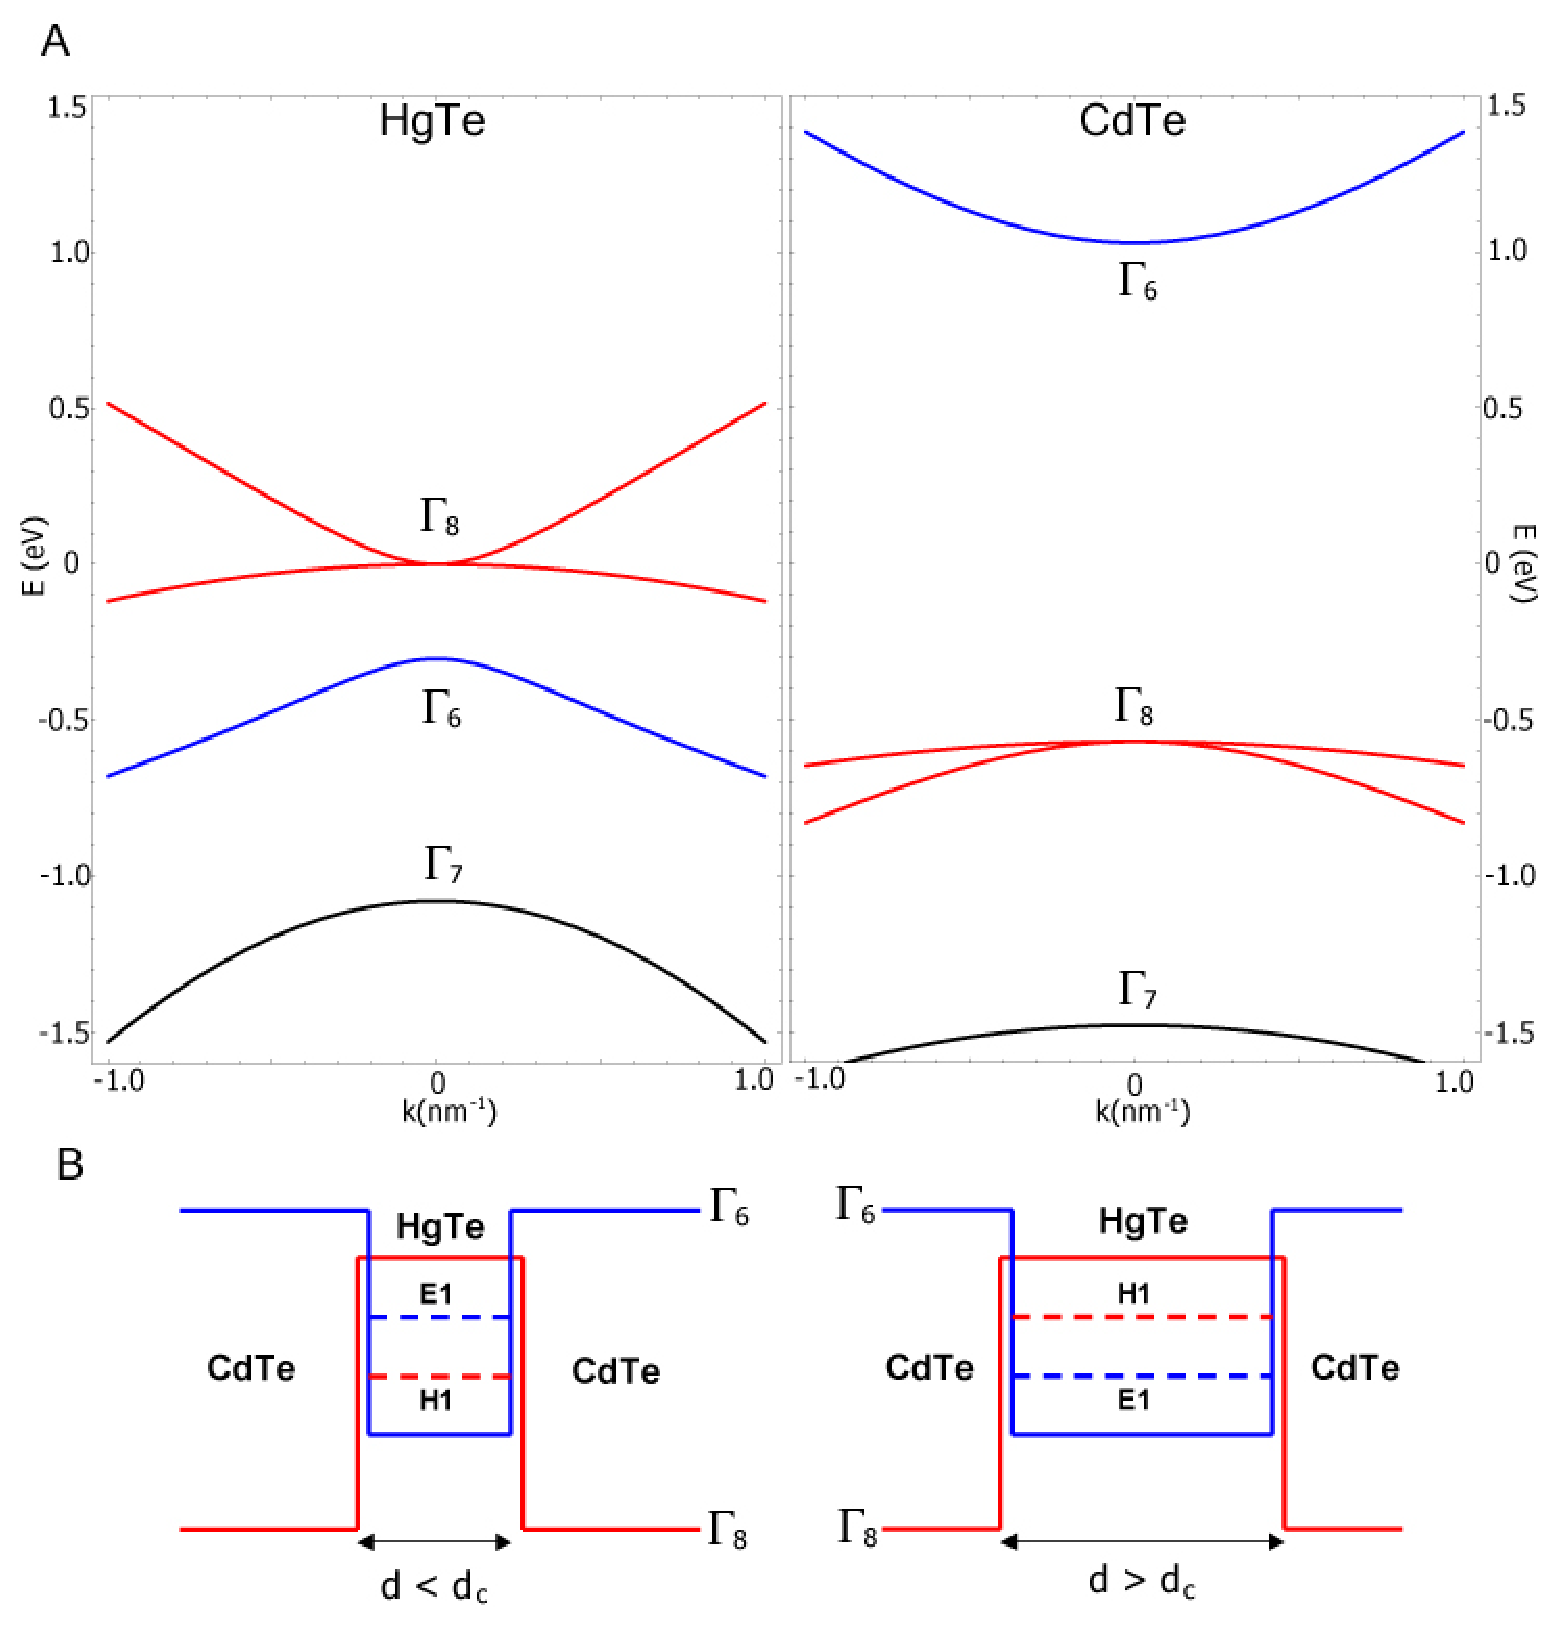
\includegraphics[scale=0.35]{pic/fig2.eps}
	\caption{A,HgTe与CdTe在布里渊区$\Gamma$点附近的体能带结构。B,CdTe/HgTe量子阱结构中正常态$d<d_c$与$d>d_c$的能级结构示意图。图片来源于文献\upcite{re3}}\label{fig2}
\end{figure}
\qquad 当一个系统哈密顿量满足TRS的时候,由Kramer定理可以知道此时每一个本征态的简并度为2,或者说满足TRS的算符,Kramer对在BZ中一定存在简并对。对于无自旋的粒子,时间反演算符为$\mathcal{T}=\mathcal{K}$,这里$\mathcal{K}$是复共轭算符 此时$\mathcal{T}^2=1$;对于有自旋的粒子,时间反演算符为$\mathcal{T}=e^{i\pi S_y}\mathcal{K}$,此时满足$\mathcal{T}^2=-1$。如图\ref{fig1}(d)所示,由于QSHE是时间反演不变的,所以它的连接价带和导带的表面态是由两支自旋动量都相反的表面态组成,而这两支表面态的交点正是时间反演不变动量点。这种表面态在实空间中的表现则如图\ref{fig1}(c)所示,系统与环境的交界面处存在着两个导电通道,其中输运方向和自旋方向都是相反的,是由时间反演对称保护的,所以电子的背散射是被禁止导致电子的无耗散运动,形成了电子输运的高速公路,正是这种特殊的性质,为将来量子器件的应用开启了新的大门。

\begin{figure}[h]
\centering
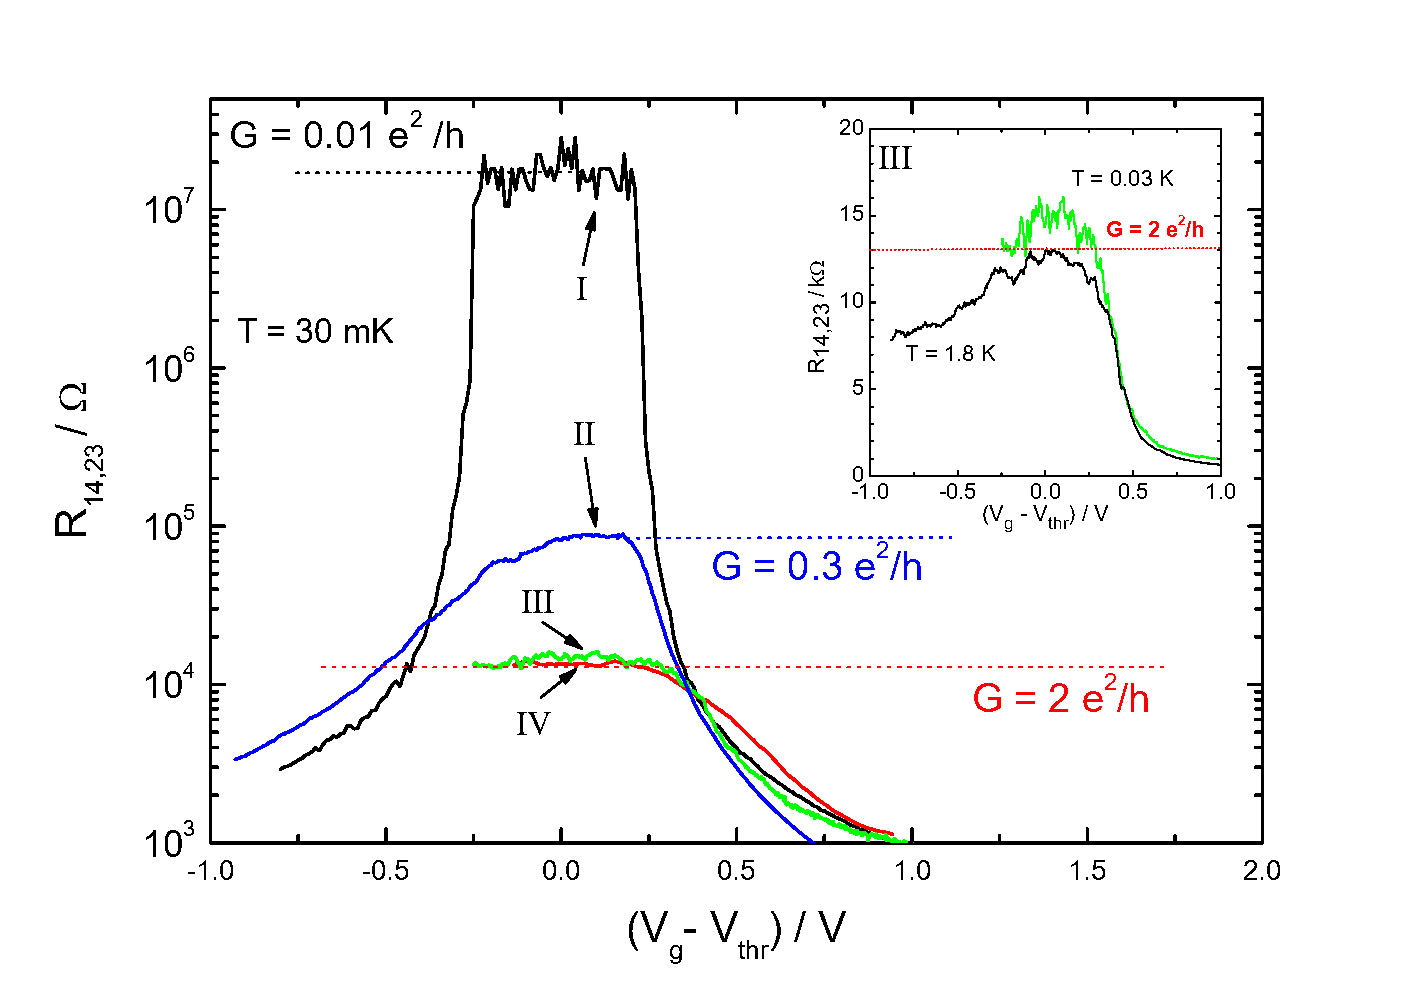
\includegraphics[scale=0.3]{pic/fig3.png}
\caption{HgTe/CdTe量子阱霍尔电阻随HgTe厚度的变化。图片来源于文献\upcite{re5}}\label{fig3}
\end{figure}
\qquad 实现拓扑绝缘体需要较强的SOC来将体态能带打开一个小的能隙,因为SOC起源于相对论效应,而元素周期表中越重的元素其相对论效应越强,则在真实材料体系中实现QSHE需要在较重的元素中搜寻。2006年张守晟等人通过理论语言在HgTe/CdTe的量子阱组成的三明治结构中,通过调节量子阱的厚度可以实现能带反转,进而实现QSHE如图\ref{fig2}\upcite{re4}。实验上很快就在CdTe/HgTe/CdTe的量子阱中通过调节HgTE的厚度,发现霍尔电导的稳定平台,且不受样品厚度等其它因素的影响如图\ref{fig3}\upcite{re5}。这是实验上首次确认了量子自旋霍尔效应。
%======================================================
\subsection{拓扑超导体}
\qquad  1911年,H.K.Onnes在研究金属汞处于极低温下的物性时,发现汞的电阻在温度降低的时候也慢慢变小,但是在温度达到4.2K时电阻突然变为0\upcite{re7},这种有着零电阻的新物态被Onnes称为超导态,并将电阻突然变为0时的温度称为超导体的转变温度(T$_c$),之后在1933年W.Meissner等人发现了除零电阻外超导体的第二种特性;完全抗磁性,即Meissner效应\upcite{re8}。零电阻和完全抗磁性是判断超导体的两个基本的判断证据。在超导现象被发现之后,科学家致力于寻找正确的微观机制来解释这一机制,直到1957 J. Bardeen,L. N. Cooper, J. R. Schrieffer三人共同提出了BCS理论\upcite{re9},从理论上成功的解释了超导现象。之后科学家发现了另外一种转变温度远大于BCS理论所预言极限的超导材料YBa$_2$Cu$_3$O$_y$(YBCO),将超导的转变温度推到了液氮沸点以上,研究人员在不断的提高超导体的转变温度的同时,也在理论上探索着这种高温超导体的形成机理\upcite{re10}。随着拓扑绝缘体在理论语言及实验验证的进展\upcite{re4,re5},因为绝缘体与描述超导体的Bogoliubov–de Gennes(BdG)哈密顿量之间的相似性,准粒子的BdG哈密顿量即对应着能带绝缘体的哈密顿量,超导体的能隙即对应着能带绝缘体的能隙, 研究人员开始关注超导体的拓扑性质\upcite{re11}。

\qquad 最简单的理解时间反演不变拓扑超导体的方式是和拓扑绝缘体进行类比,二维(2D)手性拓扑超导体是类似于量子霍尔效应的超导体,一个陈数为$N$的量子霍尔态有$N$个手性边界态,对于手性的拓扑超导体如果其拓扑量子数为$\mathcal{N}$则有$\mathcal{N}$个手性的马约拉纳边界态。因为BdG哈密顿量的正能态与负能态描述的是相同的物理自由度,所以每个马约拉纳手性边界态只有量子霍尔效应种的手性边界态一半的自由度,所以手性边界态是2D最小化的拓扑边界态。手性拓扑超导体与量子霍尔态的相似性如图\ref{fig4}上半部分所示。
\begin{figure}[h]
	\centering
	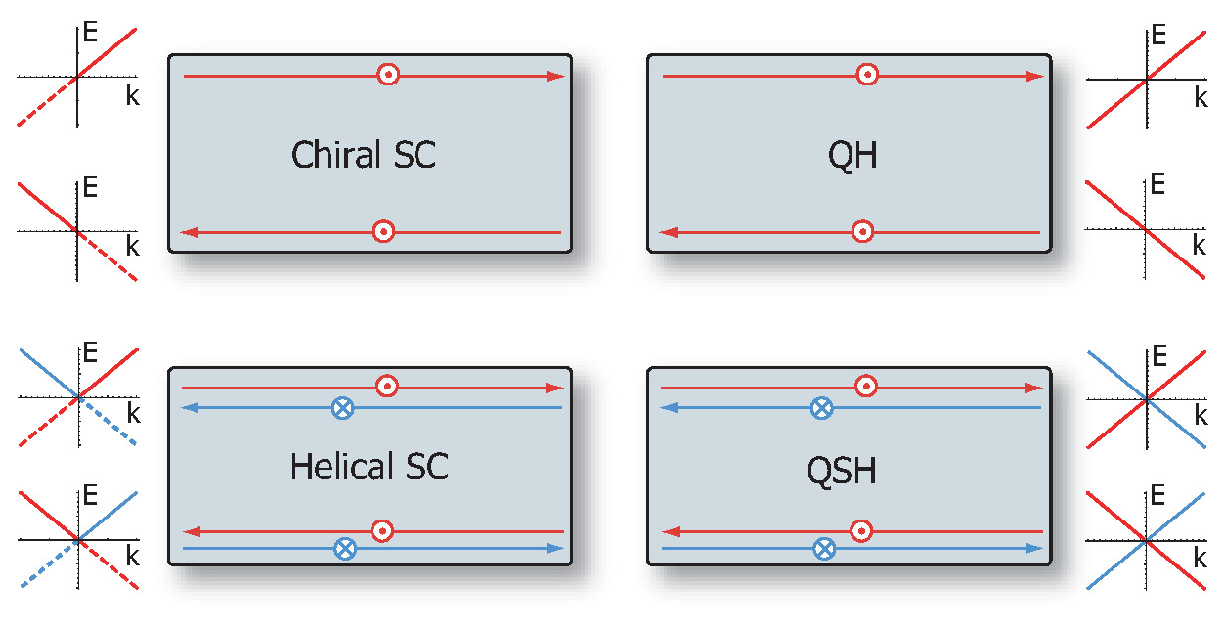
\includegraphics[scale=0.5]{pic/fig4.eps}
	\caption{(a)2D手性超导体与量子霍尔态的比较。(b)2D TRS拓扑超导体与量子自旋霍尔绝缘体比较 。图片来源于文献\upcite{re11}}\label{fig4}
\end{figure}
依照相同的逻辑,同样可以考虑和量子自旋霍尔效应类似的超导态,一个螺旋拓扑超导体,自旋向上的费米子组成$p_x+ip_y$的态,自旋向下的费米子组成$p_x-ip_y$的态。这样态存在一个边界上存在绕行方向相反的螺旋马约拉纳边界态且体态不存在能隙关闭点。相反,时间反演不变拓扑绝缘体的边界态是有两倍自由度的螺旋态Dirac费米子。对于量子自旋霍尔效应态,边界态的不能存在质量项,这是由时间反演对称保护的。因此,这样的超导相是由时间反演对称保护的,可以由$\mathit{Z}_2$拓扑不变量描述\upcite{re12}。

\qquad 2008年Fu和Kane两人提出了利用三维(3D)拓扑绝缘体的表面态近邻一个超导体,可以在外加磁场产生的Vortex中心束缚马约拉纳零能模\upcite{re19},如图\ref{fig5}(a)所示,在3D拓扑绝缘体表面放置两块分开的$s$-波超导体,对应的项为分别是$\phi$和0,如果改变其中一块超导体的位相$\phi$,则体系的能带也会随之发生改变,当$\phi=\pi$时正好对应着体态能隙关闭点,即图\ref{fig5}(b)所示。对于这样的一个异质结结构,此时系统的边界处会存在马约拉纳零能模。同样的也可以构造一个图\ref{fig5}(c)所示的三角异质结,这样通过调节相互之间的超导位相,可以实现马约拉纳零能模的控制。图\ref{fig5}(d)中灰色区域所示的即为马约拉纳零能模可以存在的区域。
\begin{figure}[h]
\centering
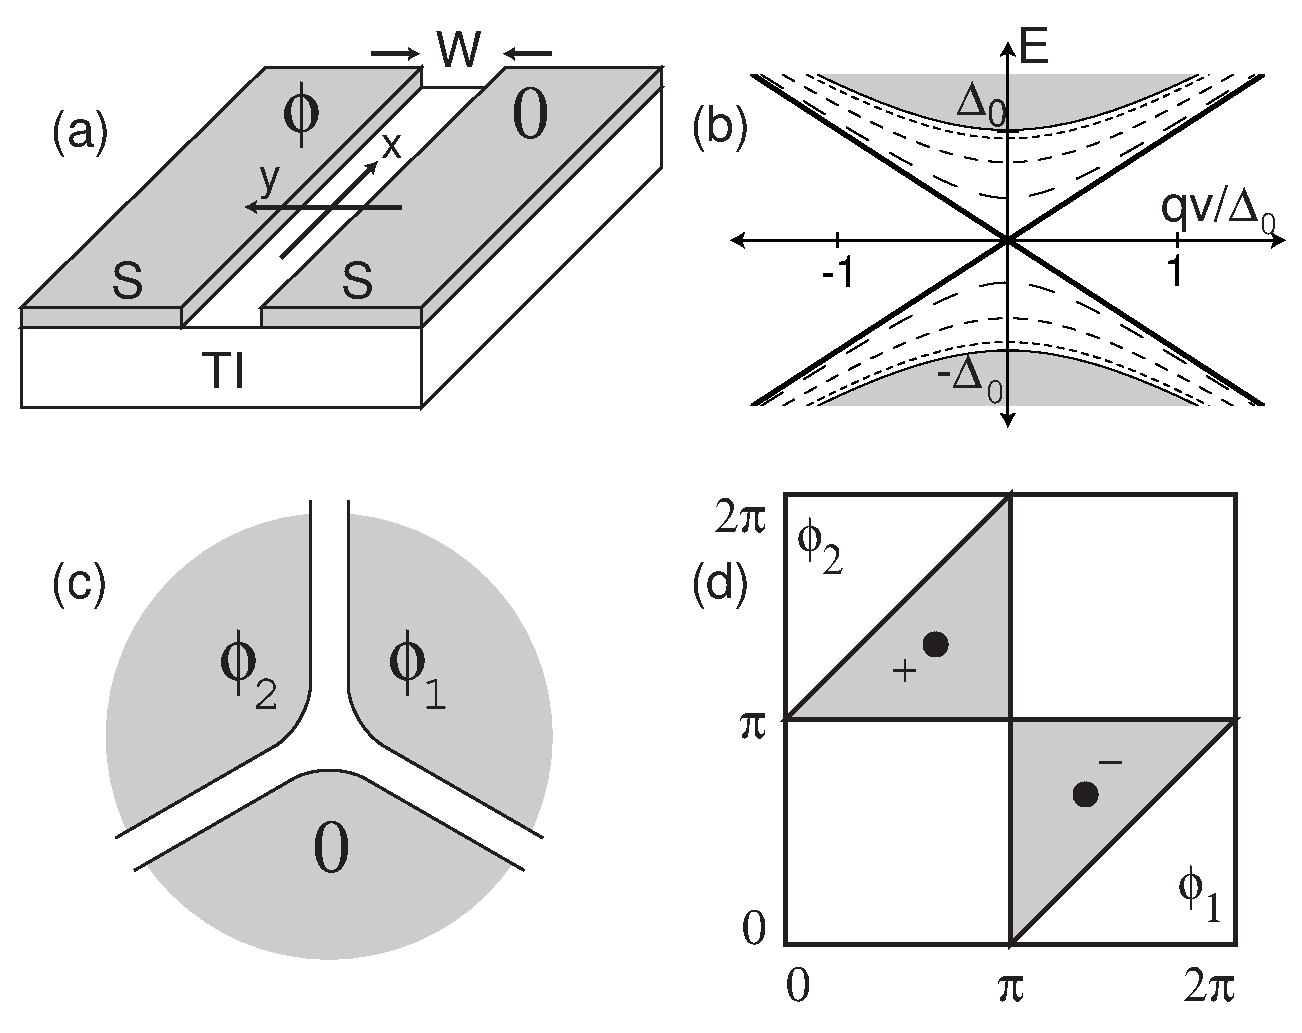
\includegraphics[scale=0.5]{pic/fig5}
\caption{(a)STIS异质结;(b)STIS线性结的能带图;(c)超导三相结;(d)三线结相图。}\label{fig5}
\end{figure}
在存在Rashba SOC的2D电子气中
\begin{equation}
H=\int d^2x\psi^\dagger\left[\mathbf{p}^2/2m+\alpha(\mathbf{\sigma}\mathbf{\times p})\cdot\hat{\mathbf{z}}-\mu\right]
\end{equation}
同样可以利用近邻效应诱导$s$-波配对,此时系统每个分立的费米面都会形成非平庸的超导体,但是两个费米面上的马约拉纳费米子会相互湮灭,所以在Rashba系统中诱导$s$-波超导配对是平庸的。之后研究人员发现通过在哈密顿量中引入破坏时间反对称的$M\sigma_z$项可以得到非平庸的超导相,它会把$\mathbf{k}=0$处的简并分离开来。如果将化学势被调节到$|\mu|<|M|$则半径较小的费米面会消失,所以仅剩下外部半径较大的费米面上诱导$s$-波超导配对,从而体系变成拓扑非平庸相\upcite{re20,re21,re22}。

\qquad 和拓扑绝缘体相同,拓扑超导体在处于拓扑相时也存在非平庸的边界态,和拓扑绝缘体不同的是在这里可以存在局域的马约拉纳费米子\upcite{re12,re13,re14,re15,re16}。马约拉纳费米子的反粒子是它本身($\gamma^\dagger=\gamma$),至今未被确认为基本粒子,但是在凝聚态体系的准粒子激发种可以产生这种粒子。相比较于其它的基本粒子,马约拉纳费米子满足非阿贝尔统计,属于非阿贝尔费米子,且其具有较好的抵抗环境噪声稳定存在,同时也具有高度非局域化性质,这两种性质在实现拓扑量子计算方面有很大的应用价值\upcite{re17,re18}。
%======================================================
\subsection{高阶绝缘体}
\qquad 最近研究人员发现了一种新的拓扑相,通常被称为高阶拓扑(HOP)\upcite{re23,re24,re25,re26,re27,re28,re29,re30,re31,re32,re33,re34,re35,re36,re37,re38,re39,re40}。对于通常的拓扑物态来说,其非平庸的边界态总是出现在比系统维度低一维的维度中,比如2D拓扑绝缘体的边界态是1维(1D)的。但是这种拓扑相其边界态出现的维度比系统维度可以低两维或者3维。一个$d$维的高阶拓扑态,它拓扑保护的无能隙边界态会出现在$d-n$维$(n\le d)$。比如一个2D$(d=2)$的HOP物态其边界态会出现的系统的角落($d=2,n=2$),3D$(d=3)$的HOP态其边界态则会出现在系统的棱$(n=2)$或者角落$(n=3)$,如图\ref{fig6}所示。
\begin{figure}[h]
\centering
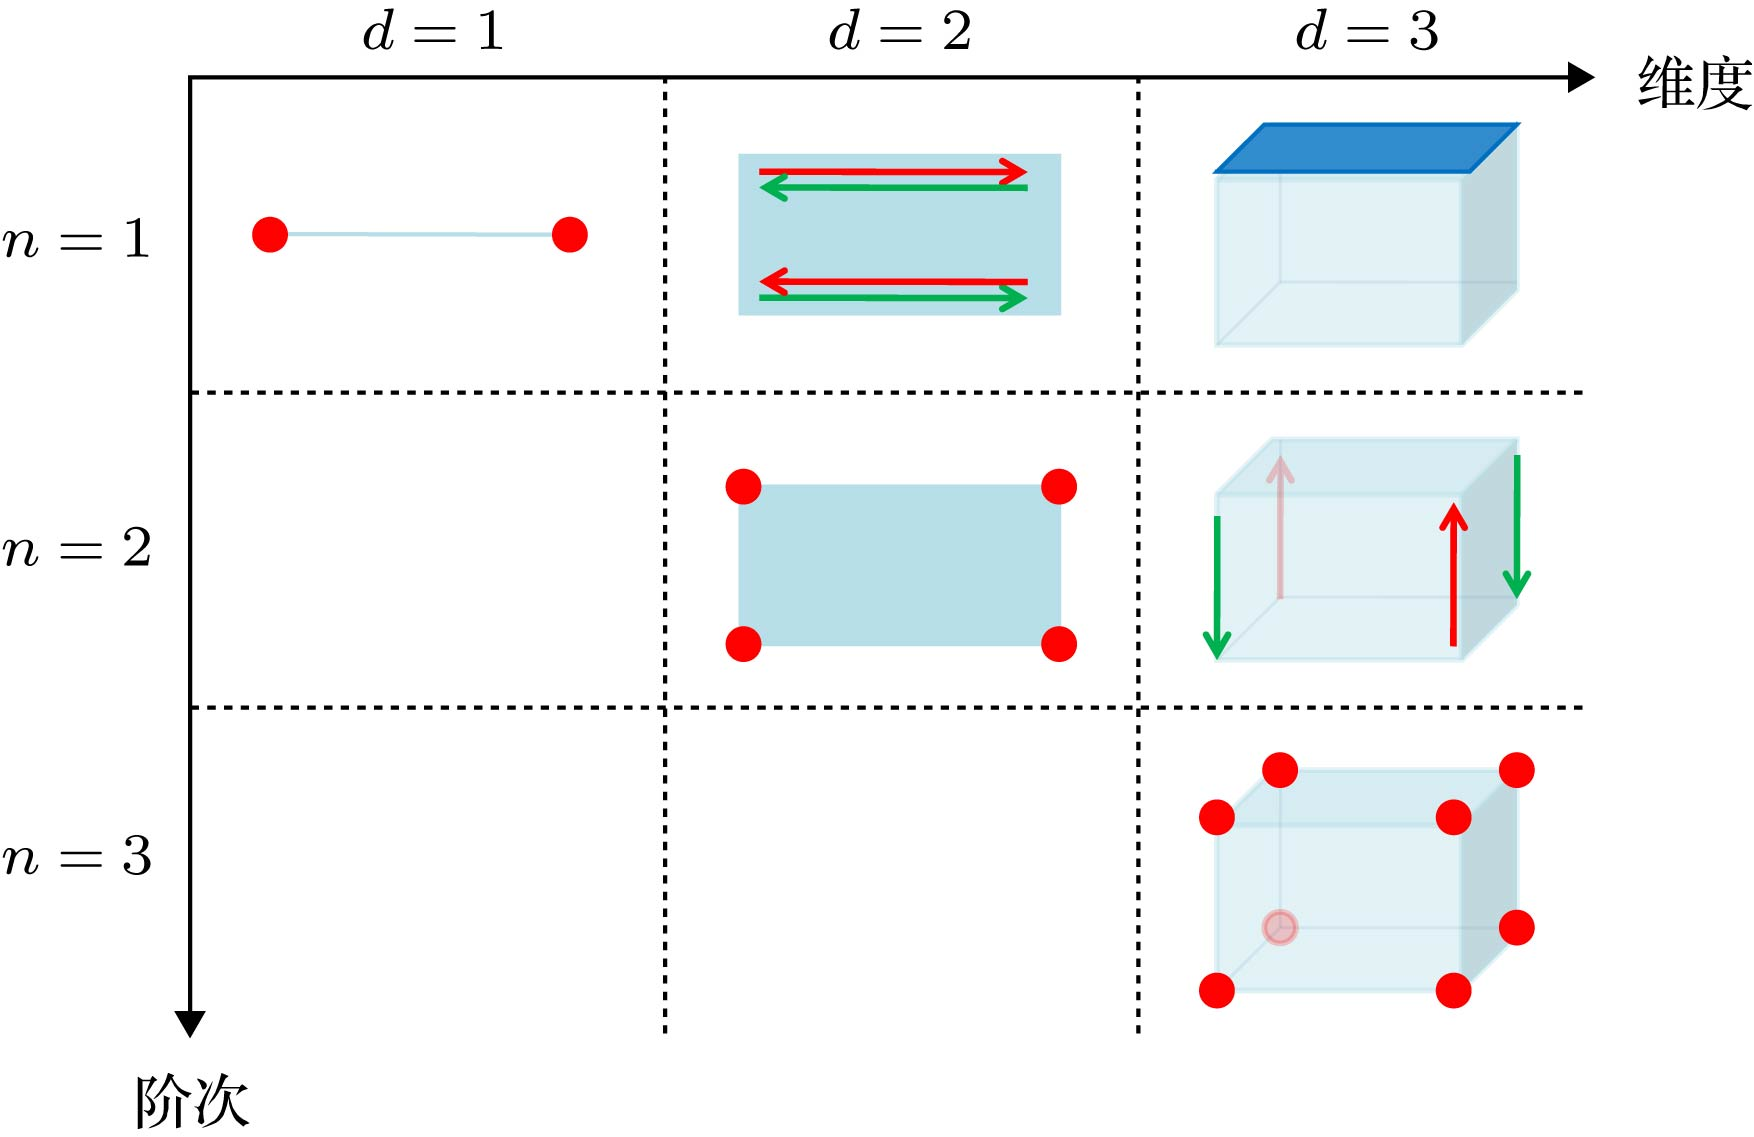
\includegraphics[scale=1.7]{pic/fig6}
\caption{拓扑物态的边界态示意图;$n=1$的行对应传统的拓扑物态, 其具有比系统维度低一维的无能隙边界态; $n\geq 2$的行对应高阶拓扑物态, 其具有比维度低n维的无能隙边界态}\label{fig6}
\end{figure}

\qquad 一个描述高阶拓扑绝缘体的四带Bloch哈密顿量为
\begin{equation}
H_c(\mathbf{k})=(M+t\sum_i\cos k_i)\tau_z\sigma_0+\Delta_1\sum_i\sin k_i\tau_x\sigma_i+\Delta_2(\cos k_x-\cos k_y)\tau_y\sigma_0\label{hoti}
\end{equation}
这里泡里矩阵$\sigma_i,\tau_i$(i=x,y,z)分别代表着自旋自由度和轨道自由度。当$1<|M|<3$且$\Delta_2=0$的时候(\ref{hoti})描述的是一阶3D拓扑绝缘体。此时哈密顿量满足时间反演对称$\mathcal{T}H_c(\mathbf{l})\mathcal{T}^{-1}=H_c(\mathbf{k})$,$\mathcal{T}=\tau_0\sigma_y\mathcal{K}$,这里$\mathcal{K}$代表复数共轭操作。当$\Delta_2=0$哈密顿量(\ref{hoti})具有$\hat{C}_4^z$旋转对称$\hat{C}_4^zH_c(\mathbf{k})(\hat{C}_4^z)^{-1}=H_c(D_{\hat{C}_4^z}\mathbf{k})$,这里旋转操作$\hat{C}_4^z\equiv \tau_0e^{-i\frac{\pi}{4}\sigma_z}$和$D_{\hat{C}_4^z}\mathbf{k}=(-k_y,k_x,k_z)$。

\qquad 正比于$\Delta_2$的这一项同时破坏了$\mathcal{T}$和$\hat{C}_4^z$对称性,但是对于它们的组合操作$\hat{C}_4^z\mathcal{T}$是反对易的
\begin{equation}
(\hat{C}_4^z\mathcal{T})H_c(\mathbf{k})(\hat{C}_4^z\mathcal{T})^{-1}=H_c(D_{\hat{C}_4^z\mathcal{T}}\mathbf{k}),\quad D_{\hat{C}_4^z\mathcal{T}}\mathbf{k}=(k_y,-k_x,-k_z)
\end{equation}
由于$\left[\hat{C}_4^z,\mathcal{T}\right]=0$,组合操作$\hat{C}_4^z\mathcal{T}$满足$(\hat{C}_4^z\mathcal{T})^4=-1$。
\begin{figure}[h]
\centering
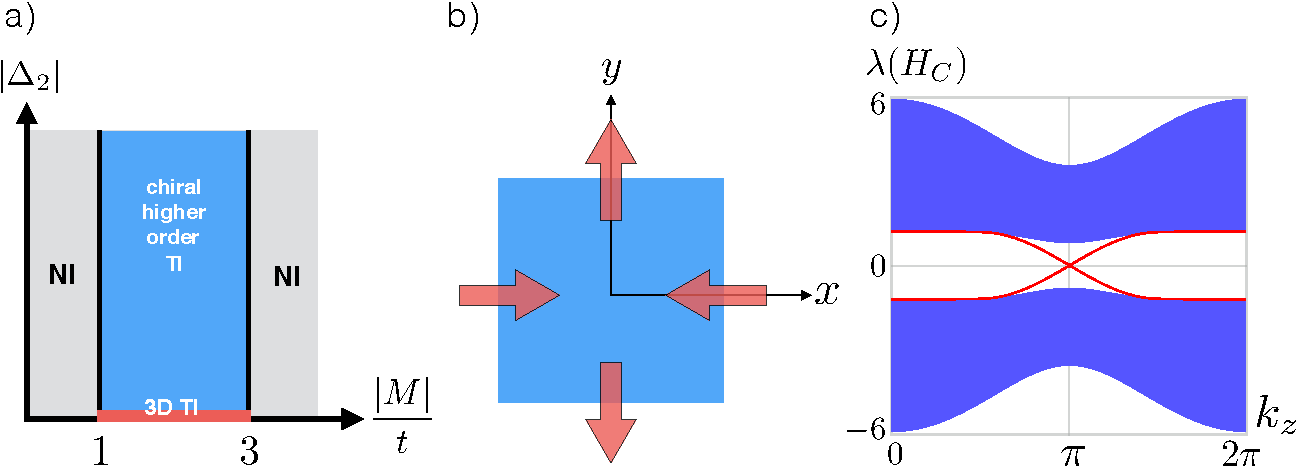
\includegraphics[scale=0.7]{pic/fig7}
\caption{手性高阶拓扑绝缘体;(a)哈密顿量(\ref{hoti})的相图,(b)一个元胞内满足$\hat{C}_4^z\mathcal{T}$的非共线反铁磁,(c)存在手性棱态(红色)的哈密顿量(\ref{hoti})的能谱图}\label{fig7}
\end{figure}
哈密顿量(\ref{hoti})的相图如图(\ref{fig7})(a)所示,当$1<|M/t|<3$且$\Delta_1,\Delta_2\neq 0$时,系统处于3D手性高阶拓扑绝缘体相。$x$和$y$方向取开边界条件,$z$方向取周期边界时,体系的能谱如图\ref{fig7}(c)所示,红色代表的手性棱模穿过了体态的能隙。从物理上讲,$\Delta_2$对应的项破坏了时间反演,对应着在$x$和$y$方向上相反的轨道流。当$\Delta_2$无限小的时候,它的主要作用是会在3D拓扑绝缘体的(100)与(010)表面上打开一个质量相反的能隙,这时候四个棱就是就会变成Dirac质量变号的质量畴壁,从而在棱上形成无能隙的手性模,也正好就是高阶拓扑绝缘体中的棱模。另外一种打破时间反演并保持$\hat{C}_4^z\mathcal{T}$的物理机制是在元胞内存在$(\pi,\pi,0)$方向上的非共线反铁磁序,如图\ref{fig7}(b)所示。这里值得注意的是,即使$\Delta_2$是有限大小的值,3D拓扑绝缘体的(001)面始终是无能隙的,由于Dirac锥是受$\hat{C}_4^z\mathcal{T}$保护的,表面在这个操作下是不变的,且存在一个Kramers类似的简并。通过第一性原理计算,研究人员同样确定SnTe在一定方向上施加压力是一种可以实现手性高阶拓扑绝缘体的材料\cite{re23}。
%======================================================
\subsection{高阶拓扑超导体}
\qquad 随着实验上在100K温度下实现了2D拓扑绝缘体\upcite{re41,re42},研究人员利用超导体的近邻效应,将2D拓扑绝缘体放置在一个高温超导体的基底上从而在拓扑绝缘体中诱导出$d$-波配对,从而来实现2D的高阶拓扑超导体\upcite{re28,re27}。与传统的一阶拓扑超导体不同的是,此时系统中马约拉纳态是处在样品的角落处的,如图\ref{fig8}所示。
\begin{figure}[h]
\centering
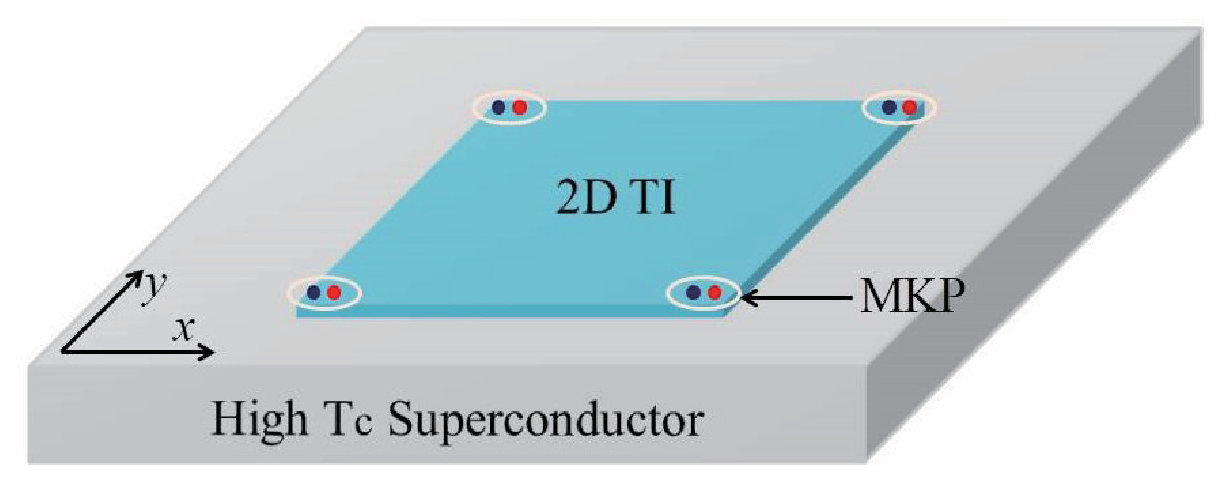
\includegraphics[scale=0.7]{pic/fig8}
\caption{示意图展示;一个2D拓扑绝缘体长在$d$-波或者$s_\pm$-波的高温超导体上,零能马约拉纳Kramers对(MKP)将会出现在2D拓扑绝缘体的角落。}\label{fig8}
\end{figure}
产生这个结果的物理图像如下:2D拓扑绝缘体的边界态是由1D无质量的Dirac费米子描述的,当通过近邻效应将2D拓扑绝缘体放置在超导体上面时,边界态会被诱导出的超导配对打开一个能隙,从而引入一个Dirac质量项。由于超导配对的对称性(比如说$d$-波配对),在每个角落处诱导出的质量是相反的,所以在系统的每个角落处形成类似质量畴壁的MKP激发。

\qquad 根据上面的解释,这个结果的主要来源就是边界态,那么从一个2D拓扑绝缘体模型出发,之后通过近邻在2D拓扑绝缘体上诱导超导配对来进行研究。BdG哈密顿量写为
\begin{equation}
\begin{aligned}
\hat{H}&=\sum_\mathbf{k}\Psi_\mathbf{k}^\dagger H(\mathbf{k})\Psi_\mathbf{k}\\
\Psi^\dagger_\mathbf{k}&=(c^\dagger_{a\uparrow\mathbf{k}},c^\dagger_{b\uparrow\mathbf{k}},c^\dagger_{a\downarrow\mathbf{k}},c^\dagger_{b\downarrow\mathbf{k}},c_{a\downarrow\mathbf{-k}},c_{b\downarrow\mathbf{-k}},c_{a\uparrow\mathbf{-k}},c_{b\uparrow\mathbf{-k}})
\end{aligned}
\end{equation}
\begin{equation}
\begin{aligned}
H(\mathbf{k})&=M(\mathbf{k})\sigma_z\tau_z+A_x\sin k_x\sigma_xs_z+A_y\sin k_y\sigma_y\tau_z+\Delta(\mathbf{k})s_y\tau_y-\mu\tau_z\\\label{hoti2}
\end{aligned}
\end{equation}
这里泡里矩阵$s_i,\sigma_i,\tau_i$分别在自旋空间($\uparrow,\downarrow$),轨道空间(a,b),和粒子空穴空间。质量项$M(\mathbf{k})=m_0-t_x\cos k_x-t_y\cos k_y$,和$A_{x/y}$代表动能项代表着动能,$\Delta(\mathbf{k})$是超导配对,$\mu$是化学势。对于高温超导体,将配对取为
\begin{equation}
\Delta(\mathbf{k})=\Delta_x+\Delta_x\cos k_x+\Delta_y\cos k_y
\end{equation}
这个形式可以同时描述$d$-波和$s_\pm$-波这两种不同的配对形式。哈密顿量(\ref{hoti2})具有时间反演对称$\mathcal{T}H(\mathbf{k})\mathcal{T}^{-1}=H(-\mathbf{k})$,时间反演算符为$\mathcal{T}=is_y\mathcal{K}$,同时也满足粒子空穴对称$\mathcal{C}H(\mathbf{k})\mathcal{C}^{-1}=-H(-\mathbf{k})$,粒子空穴算符$\mathcal{C}=\tau_x\mathcal{K}$,$\mathcal{K}$代表复数共轭操作。

\qquad 接下来考虑铜基超导体中的$d$-波配对
\begin{equation}
\Delta_0=0,\qquad\Delta_x=-\Delta_y\equiv\Delta_d
\end{equation}
将哈密顿量$x$方向取开边界条件$y$方向取周期性边界条件(圆柱体结构),计算得到的能谱如图\ref{fig9}(a)所示,可以看到2D拓扑绝缘体的螺旋边界态在诱导出超导配对之后打开一个能隙,而从实空间的计算结果\ref{fig9}(b)也可以看到,系统的每个角落处都局域一个MKP,其能量由于粒子空穴对称性的存在被限制在零能处。
\begin{figure}[h]
\centering
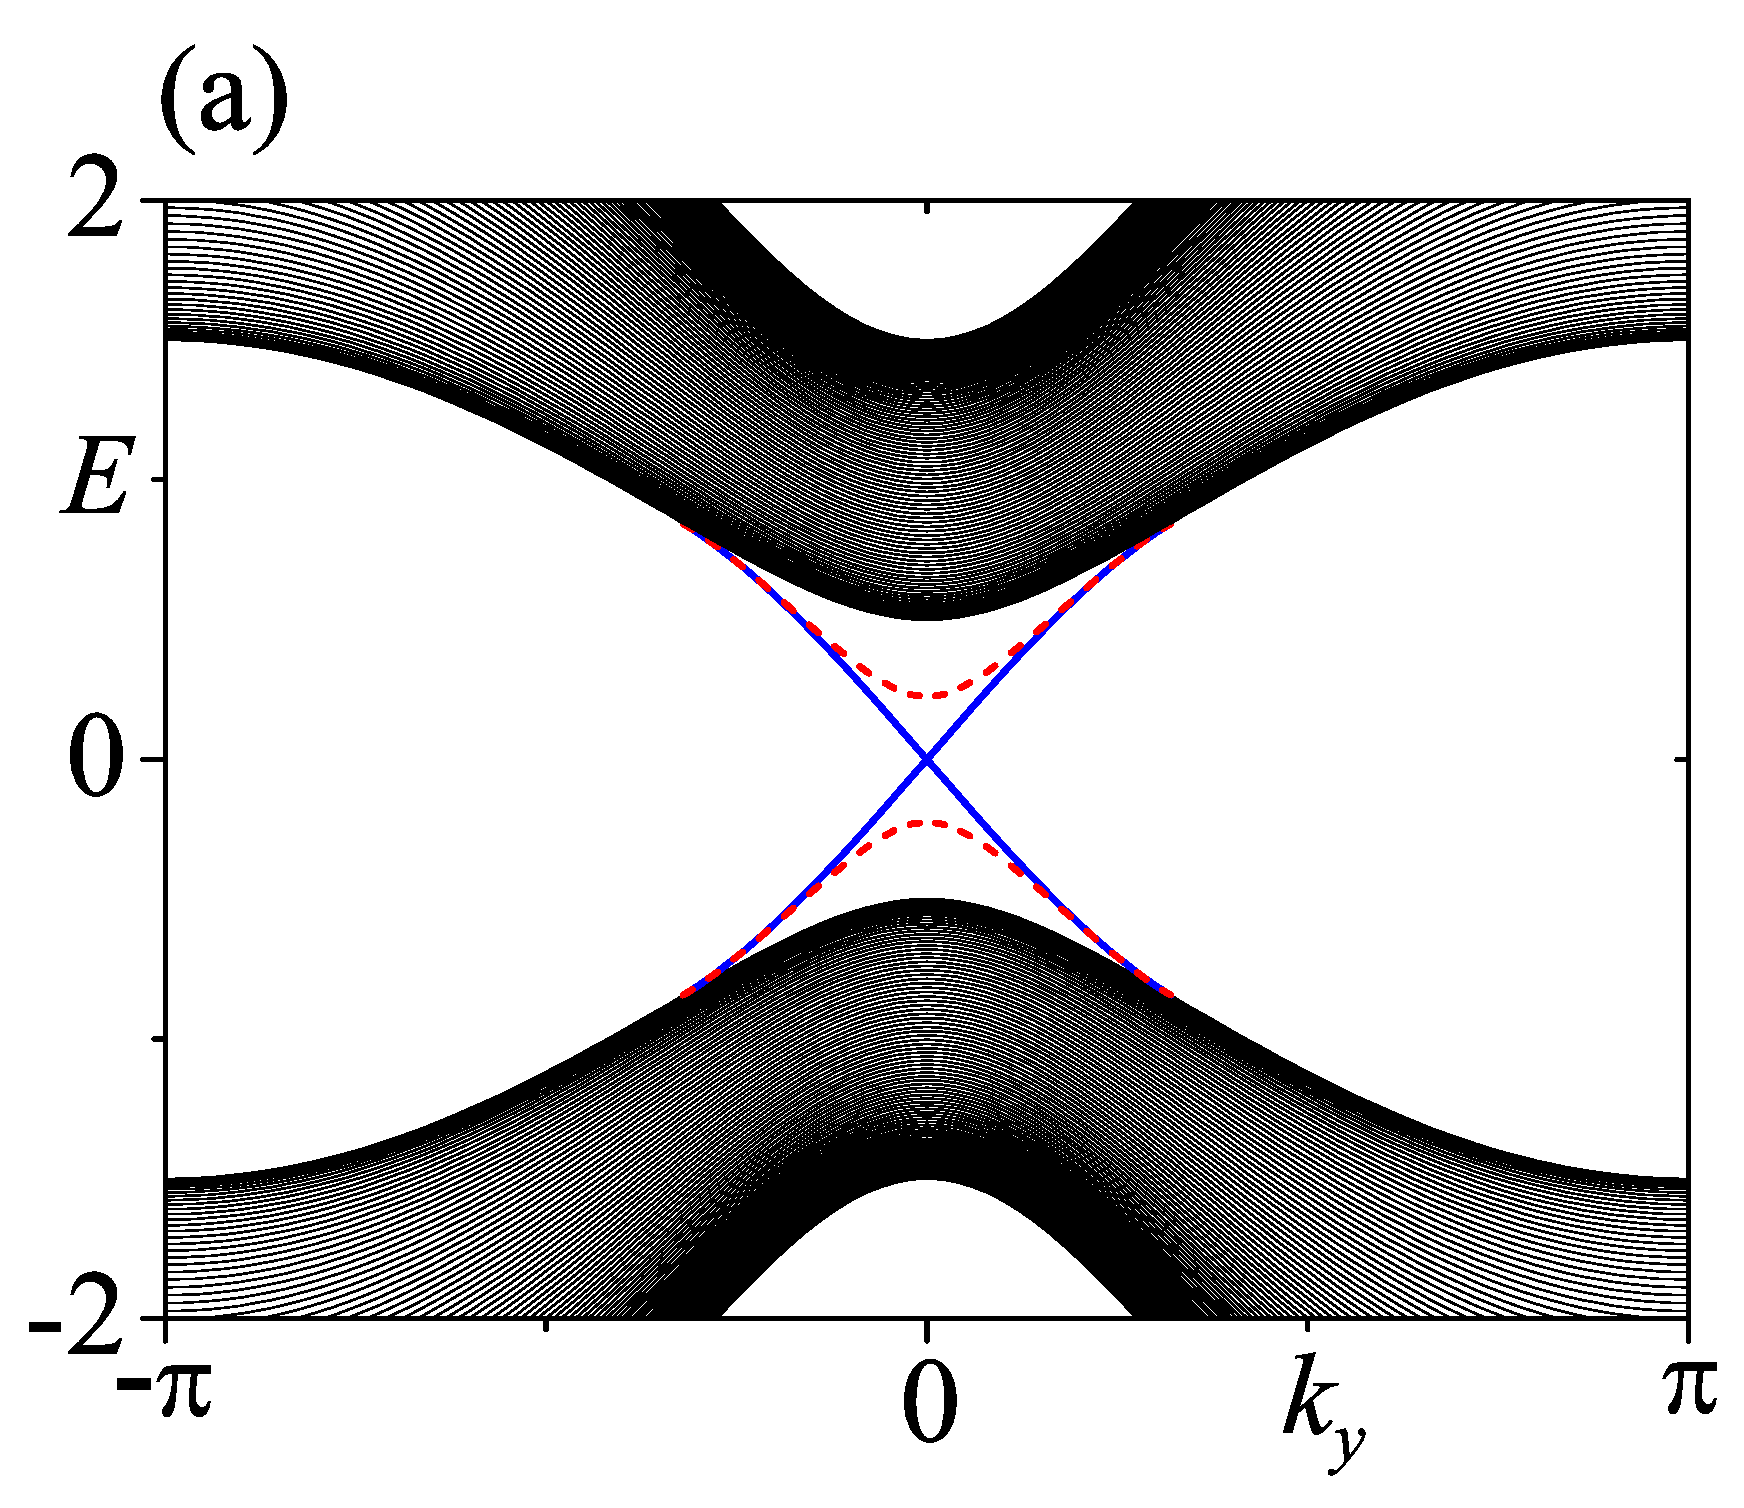
\includegraphics[scale=0.26]{pic/fig9}
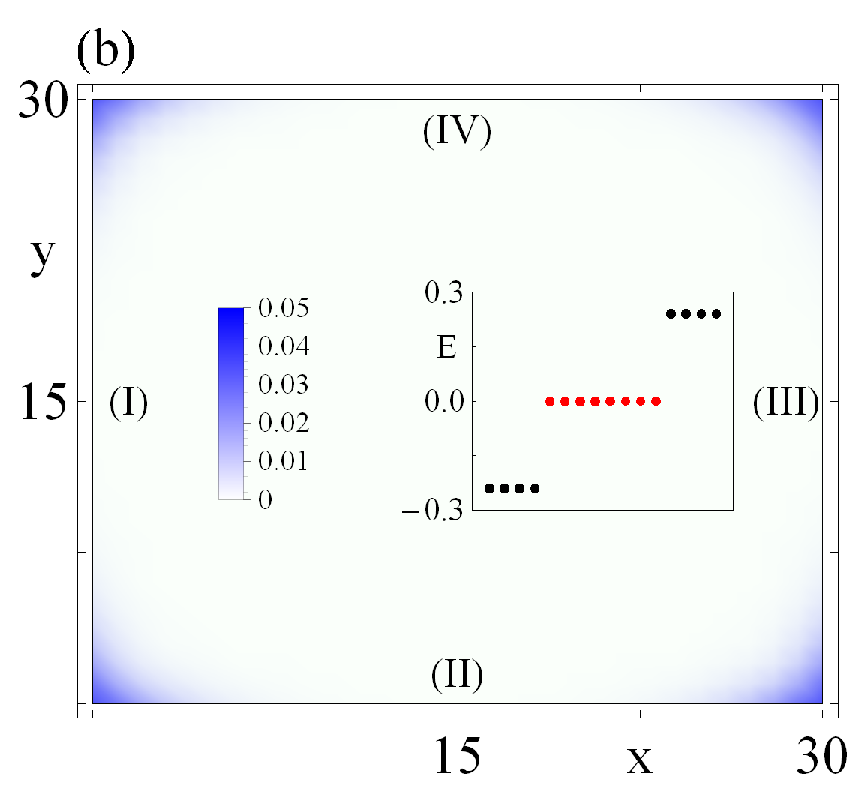
\includegraphics[scale=0.5]{pic/fig10}
\caption{(a)圆柱体结构能谱图;(b)四个MKP的波函数分布}\label{fig9}
\end{figure}
有趣的是,此时马约拉纳零能态并不是出现的vortex中间或者是原子链尾端,它出现在了2D系统的角落,这正是最近研究人员提出的高阶拓扑绝缘体以及高阶拓扑超导体的特征。这里晶体的对称性是被强调了的,但是现在这个体系出现角态并不依赖于晶体的对称性。这里需要提及的是,体态的$d$-波超导配对是有节点存在的($\Delta(\mathbf{k})=0$),MKP将会与这些无能隙的模混合到一起,但是仍然可以利用STM进行观测,当隧穿电导在电压等于零的位置出现一个明显的电导峰的时候,即为有力的证据。

\qquad 解析来通过有效边界理论来得到一个更加直观的物理图像,首先将哈密顿量(\ref{hoti2})在$\Gamma=(0,0)$处做低能展开,并保留到二阶
\begin{equation}
H(\mathbf{k})=(m+\frac{t_x}{2}k_x^2+\frac{t_y}{2}k_y^2)\sigma_z\tau_z+\lambda_xk_x\sigma_xs_z+\lambda_yk_y\sigma_y\tau_z-\frac{1}{2}(\Delta_xk_x^2+\Delta_yk_y^2)s_y\tau_y\label{hoti2e}
\end{equation}
对于$d$-波超导体有$\Delta_x+\Delta_y=0$,对于2D拓扑绝缘体$m=m_0-t_x-t_y<0$保证在在没有超导配对的时候体系处于拓扑非平庸相。如图\ref{fig9}(b)所示,将正方形的四个边分别标记为(\uppercase\expandafter{\romannumeral1}),(\uppercase\expandafter{\romannumeral2}),(\uppercase\expandafter{\romannumeral3}),(\uppercase\expandafter{\romannumeral4}),这里先关注(\uppercase\expandafter{\romannumeral1})这条边,取$x$方向在实空间$k_x\rightarrow-i\partial_x$,将哈密顿量(\ref{hoti2e})分解成两部分$H=H_0+H_p$
\begin{equation}
\begin{aligned}
H_0(-i\partial_x,k_y)&=(m-t_x\partial_x^2/2)\sigma_z\tau_z-i\lambda_x\sigma_xs_z\partial_x\\
H_p(-i\partial_x,k_y)&=\lambda_yk_y\sigma_y\tau_z+\frac{\Delta_y}{2}s_y\tau_y\partial_x^2
\end{aligned}
\end{equation}
在这里忽略了$k_y^2$项,首先需要求解$H_0$的本征方程,然后将$H_p$当作微扰,所以$k_y^2$的贡献自然是可以忽略的。

\qquad 在边界条件$\psi_\alpha(0)=\psi_\alpha(\infty)$下来求解$H_0\psi_\alpha(x)=E_\alpha\psi_\alpha(x)$可以得到四个零能解,其形式为
\begin{equation}
\psi_\alpha(x)=\mathcal{N}_x\sin(\kappa_1x)e^{-\kappa_2x}e^{ik_yy}\xi_\alpha
\end{equation}
归一化系数为 $|\mathcal{N}_x|^2=4|\kappa_2(\kappa_1^2+\kappa_2^2)/\kappa_1^2|$。(符号简记,$\kappa_1=\sqrt{|(2m_x/t_x)|-(\lambda_x^2/t_x^2)}$,$ \kappa_2=(\lambda_x/t_x)$)。旋量部分 $\xi_\alpha$ 满足 $\sigma_ys_z\tau_z=-\xi_\alpha$,可以将旋量部分选取为
\begin{equation}
\begin{aligned}
\xi_1&=|\sigma_y=-1\rangle\otimes|\uparrow\rangle\otimes|\tau=+1\rangle\\
\xi_2&=|\sigma_y=+1\rangle\otimes|\downarrow\rangle\otimes|\tau=+1\rangle\\
\xi_3&=|\sigma_y=+1\rangle\otimes|\uparrow\rangle\otimes|\tau=-1\rangle\\
\xi_4&=|\sigma_y=-1\rangle\otimes|\downarrow\rangle\otimes|\tau=-1\rangle
\end{aligned}
\end{equation}
在这个基矢的选取下,微扰部分$H_p$计算为
\begin{equation}
H_{\uppercase\expandafter{\romannumeral1},\alpha\beta}(k_y)=\int_{0}^{\infty}dx\psi^*_\alpha(x)H_p(-i\partial_x,k_y)\psi_\beta(x);
\end{equation}
最后得到有效哈密顿量为
\begin{equation}
H_{\uppercase\expandafter{\romannumeral1}}(k_y)=-A_yk_ys_z+M_{\uppercase\expandafter{\romannumeral1}}s_y\tau_y
\end{equation}
这里
\begin{equation}
M_{\uppercase\expandafter{\romannumeral1}}=\frac{\Delta_x}{2}\int_{0}^{\infty}dx\psi_\alpha^*(x)\partial_x^2\psi_\alpha(x)=\Delta_x\frac{m}{t_x}
\end{equation}
其它三个边界上的有效哈密顿量也可以通过相似方式求解得到,结果为
\begin{equation}
\begin{aligned}
H_{\uppercase\expandafter{\romannumeral1}}&=-A_yk_ys_z+M_{\uppercase\expandafter{\romannumeral1}}s_y\tau_y\\
H_{\uppercase\expandafter{\romannumeral2}}&=A_xk_xs_z+M_{\uppercase\expandafter{\romannumeral2}}s_y\tau_y\\
H_{\uppercase\expandafter{\romannumeral3}}&=A_yk_ys_z+M_{\uppercase\expandafter{\romannumeral3}}s_y\tau_y\\
H_{\uppercase\expandafter{\romannumeral4}}&=-A_xk_xs_z+M_{\uppercase\expandafter{\romannumeral4}}s_y\tau_y\\\label{edge1}
\end{aligned}
\end{equation}
每条边界上的质量项满足$M_{\uppercase\expandafter{\romannumeral2}}=M_{\uppercase\expandafter{\romannumeral4}}=\Delta_ym/t_y$,$M_{\uppercase\expandafter{\romannumeral1}}=M_{\uppercase\expandafter{\romannumeral3}}=\Delta_xm/t_x$。
这里以逆时针方向为绕行正方向,可以将低能边界理论整理为
\begin{equation}
H_{\mathrm{edge}}=-iA(l)s_z\partial_l+M(l)s_y\tau_y\label{edge2}
\end{equation}

这里的动能系数$A(l)$与Dirac质量项$M(l)$都是阶跃函数:$A(l)=A_y,A_x,A_y,A_x$,$M(l)=\Delta_dm/t_x,-\Delta_dm/t_y,\Delta_dm/t_x,-\Delta_dm/t_y$($l=\mathrm{\uppercase\expandafter{\romannumeral1},\uppercase\expandafter{\romannumeral2},\uppercase\expandafter{\romannumeral3},\uppercase\expandafter{\romannumeral4}}$)。从这里可以看出,在系统的每个角落,系数$A_{x,y}$并不会改变符号,但是Dirac质量项$M_(l)$因为$d$-波配对$\Delta_x=-\Delta_y$的原因,在每个角落的位置都会反号,从而在每个角落处产生一个质量畴壁,形成类似于Jackiw-Rebbi零能模\cite{re43,re44}的束缚态。例如在边界($\mathrm{\uppercase\expandafter{\romannumeral1}}$)与($\mathrm{\uppercase\expandafter{\romannumeral2}}$)形成的角落中,零能束缚态波函数为
\begin{equation}
|\Psi^\pm_{\mathrm{MKP}}\rangle\sim e^{-\int^ldl^{'}M(l^{'})/A(l^{'})}|s_x=\tau_y=1\rangle
\end{equation}
由于哈密顿量满足时间反演不变,它保证了这两个零能态之间不会相互耦合并产生能隙。

\qquad 现在考虑另外一种配对形式的铁基高温超导体,其配对形式有$s_\pm$-波配对,实验上也观测到这种配对在费米面上当靠近BZ中心与BZ边界的时候都具有$s$-波配对的性质,但是在这两个区域内的配对符号则是相反的,当费米面与超导配对为零的节线不相交的时候,超导配对在整个体态都是有能隙的。$s_\pm$-波配对的一个简单形式为
\begin{equation}
\Delta(\mathbf{k})=\Delta_0-\Delta_1(\cos k_x+\cos k_y)
\end{equation}
这里$0\le\Delta_0\le2\Delta_1$,超导配对节线位置为$\cos k_x+\cos k_y=\Delta_0/\Delta_1$,如图\ref{fig10}所示
\begin{figure}[h]
\centering
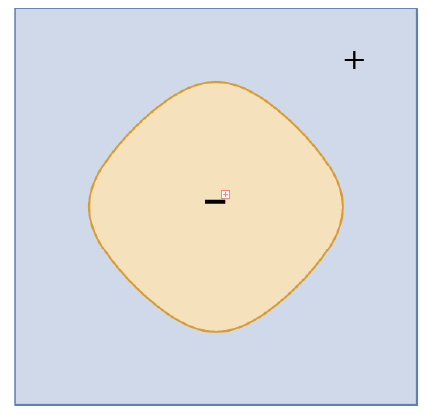
\includegraphics[scale=0.5]{pic/fig11.png}
\caption{BZ中$s_\pm$-波示意图,在靠近中心区域配对是负的,在BZ边界区域配对是正的。}\label{fig10}
\end{figure}
同样的,在$s_\pm$-波配对的情形下,可以来研究低能边界理论,将哈密顿量在$\Gamma=(0,0)$点做展开
\begin{equation}
H(\mathbf{k})=(m+\frac{t_x}{2}k_x^2+\frac{t_y}{2}k_y^2)\sigma_z\tau_z+\lambda_xk_x\sigma_xs_z+\lambda_yk_y\sigma_y\tau_z+\left[\Delta_0-2\Delta_1+\frac{\Delta_1}{2}(k_x^2+k_y^2)\right]s_y\tau_y\label{hoti2s}
\end{equation}
利用和前面相似的方法,对边界(\uppercase\expandafter{\romannumeral1})将哈密顿量分解为$H=H_0+H_p$
\begin{equation}
\begin{aligned}
H_0(-i\partial_x,k_y)&=(m-t_x\partial_x^2/2)\sigma_z\tau_z-i\lambda_x\sigma_xs_z\partial_x\\
H_p(-i\partial_x,k_y)&=\lambda_yk_y\sigma_y\tau_z+\left[\Delta_0-2\Delta_1-(\Delta_1/2)\partial_x^2\right]s_y\tau_y
\end{aligned}
\end{equation}
$H_0$的四个零能本征解与前面类似,在这四个零能的子空间中$H_p$的有效形式为
\begin{equation}
\begin{aligned}
H_{\mathrm{\uppercase\expandafter{\romannumeral1}}}(k_y)&=-A_yk_ys_z+M_{\mathrm{\uppercase\expandafter{\romannumeral1}}}s_y\tau_y\\
M_{\mathrm{\uppercase\expandafter{\romannumeral1}}}&=\int_{0}^\infty dx\Psi_\alpha^{*}(x)\left[\Delta_0-2\Delta_1-(\Delta_1/2)\partial_x^2\right]\Psi_\alpha(x)\\&=\Delta_0-2\Delta_1-\Delta_1\frac{m}{t_x}
\end{aligned}
\end{equation}
其它边界上的低能有效哈密顿量与(\ref{edge1})类似,$M_{\mathrm{\uppercase\expandafter{\romannumeral3}}}=M_{\mathrm{\uppercase\expandafter{\romannumeral1}}}=\Delta_1m/t_x$,$M_{\mathrm{\uppercase\expandafter{\romannumeral2}}}=M_{\mathrm{\uppercase\expandafter{\romannumeral4}}}$\\$=\int_{0}^{\infty}dy\Psi_\alpha^{*}(y)\left[\Delta_0-2\Delta_1-(\Delta_1/2)\partial^2_y\right]\Psi_\alpha=\Delta_0-2\Delta_1-\Delta_1m/t_y$。利用类似于(\ref{edge2})的边界坐标$l$同样可以得到每条边界上的$A(l)$是相同的,但是Dirac质量项$M(l)$是不一样的,对边界(\uppercase\expandafter{\romannumeral1}),(\uppercase\expandafter{\romannumeral2}),(\uppercase\expandafter{\romannumeral3}),(\uppercase\expandafter{\romannumeral4})其对应的质量项为$M(l)=-\bar{\Delta}_0-\Delta_1m/t_x,-\bar{\Delta
}_0-\Delta_1m/t_y,-\bar{\Delta}_0-\Delta_1m/t_x,-\bar{\Delta}_0-\Delta_1m/t_y$,这里$\bar{\Delta}_0=2\Delta_1-\Delta_0$。

\qquad 要保证在每个拐角处都可以形成MKP,那么相邻边上的Dirac质量需要改变符号,即满足下面的条件
\begin{equation}
(\bar{\Delta}_0+\Delta_1m/t_x)(\bar{\Delta}_0+\Delta_1m/t_y)<0\label{ring1}
\end{equation}
定义$R_s\equiv\sqrt{2\bar{\Delta}_0/\Delta_1}$,它代表着超导配对节线的半径,当越过这个节线的时候,配对要变号;$R_x\equiv\sqrt{-2m/t_x},R_y\equiv\sqrt{-2m/t_y}$则表示$m+(t_x/2)k_x^2+(t_y/2)k_y^2=0$(这是能带反转环,即$\sigma_z$项在越过这个环时符号会发生改变)。所以零能模存在条件(\ref{ring1})在化学势$\mu=0$的时候变为
\begin{equation}
(R_s-R_x)(R_s-R_y)<0
\end{equation}
也就意味着此时超导配对节线环需要和能带反转环相交才可以,如图\ref{fig11}所示
\begin{figure}
\centering
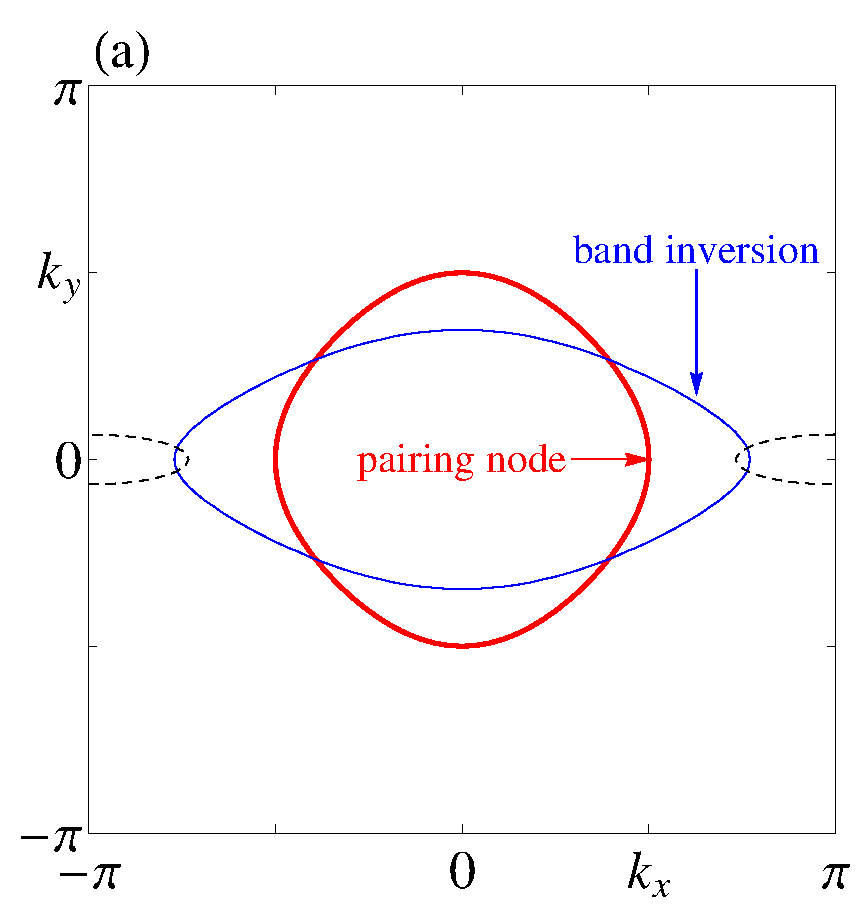
\includegraphics[scale=0.45]{pic/fig12a}
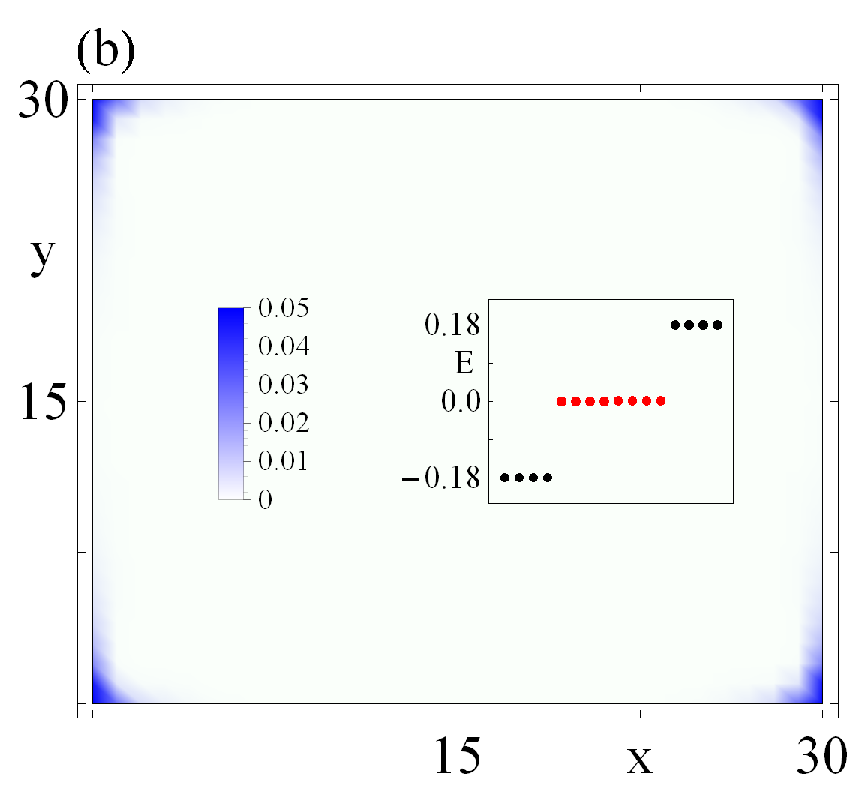
\includegraphics[scale=0.45]{pic/fig12b}
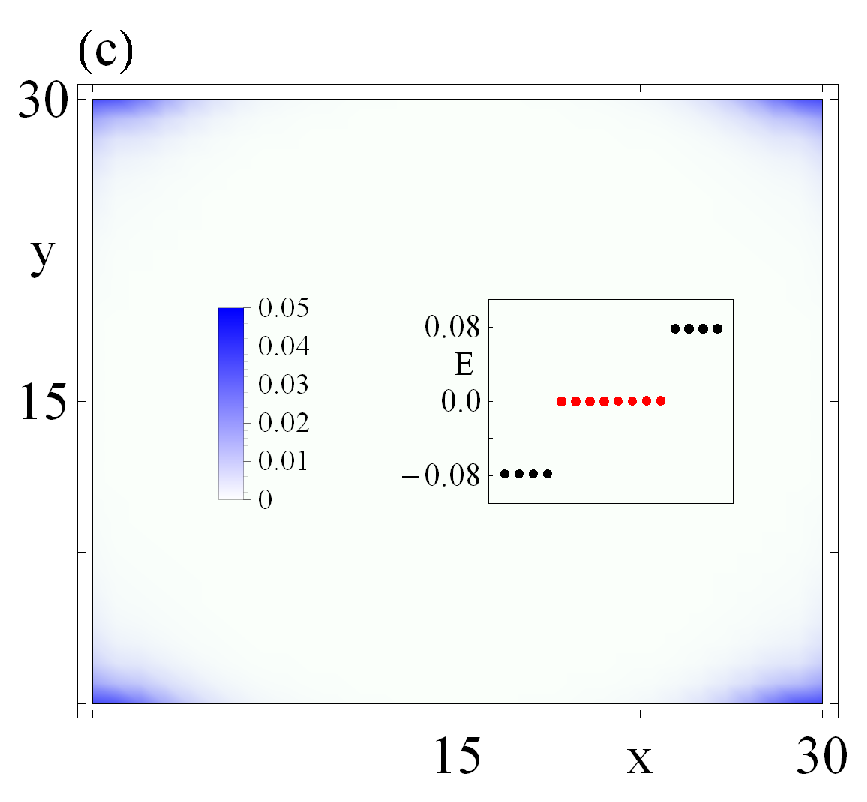
\includegraphics[scale=0.45]{pic/fig12c}
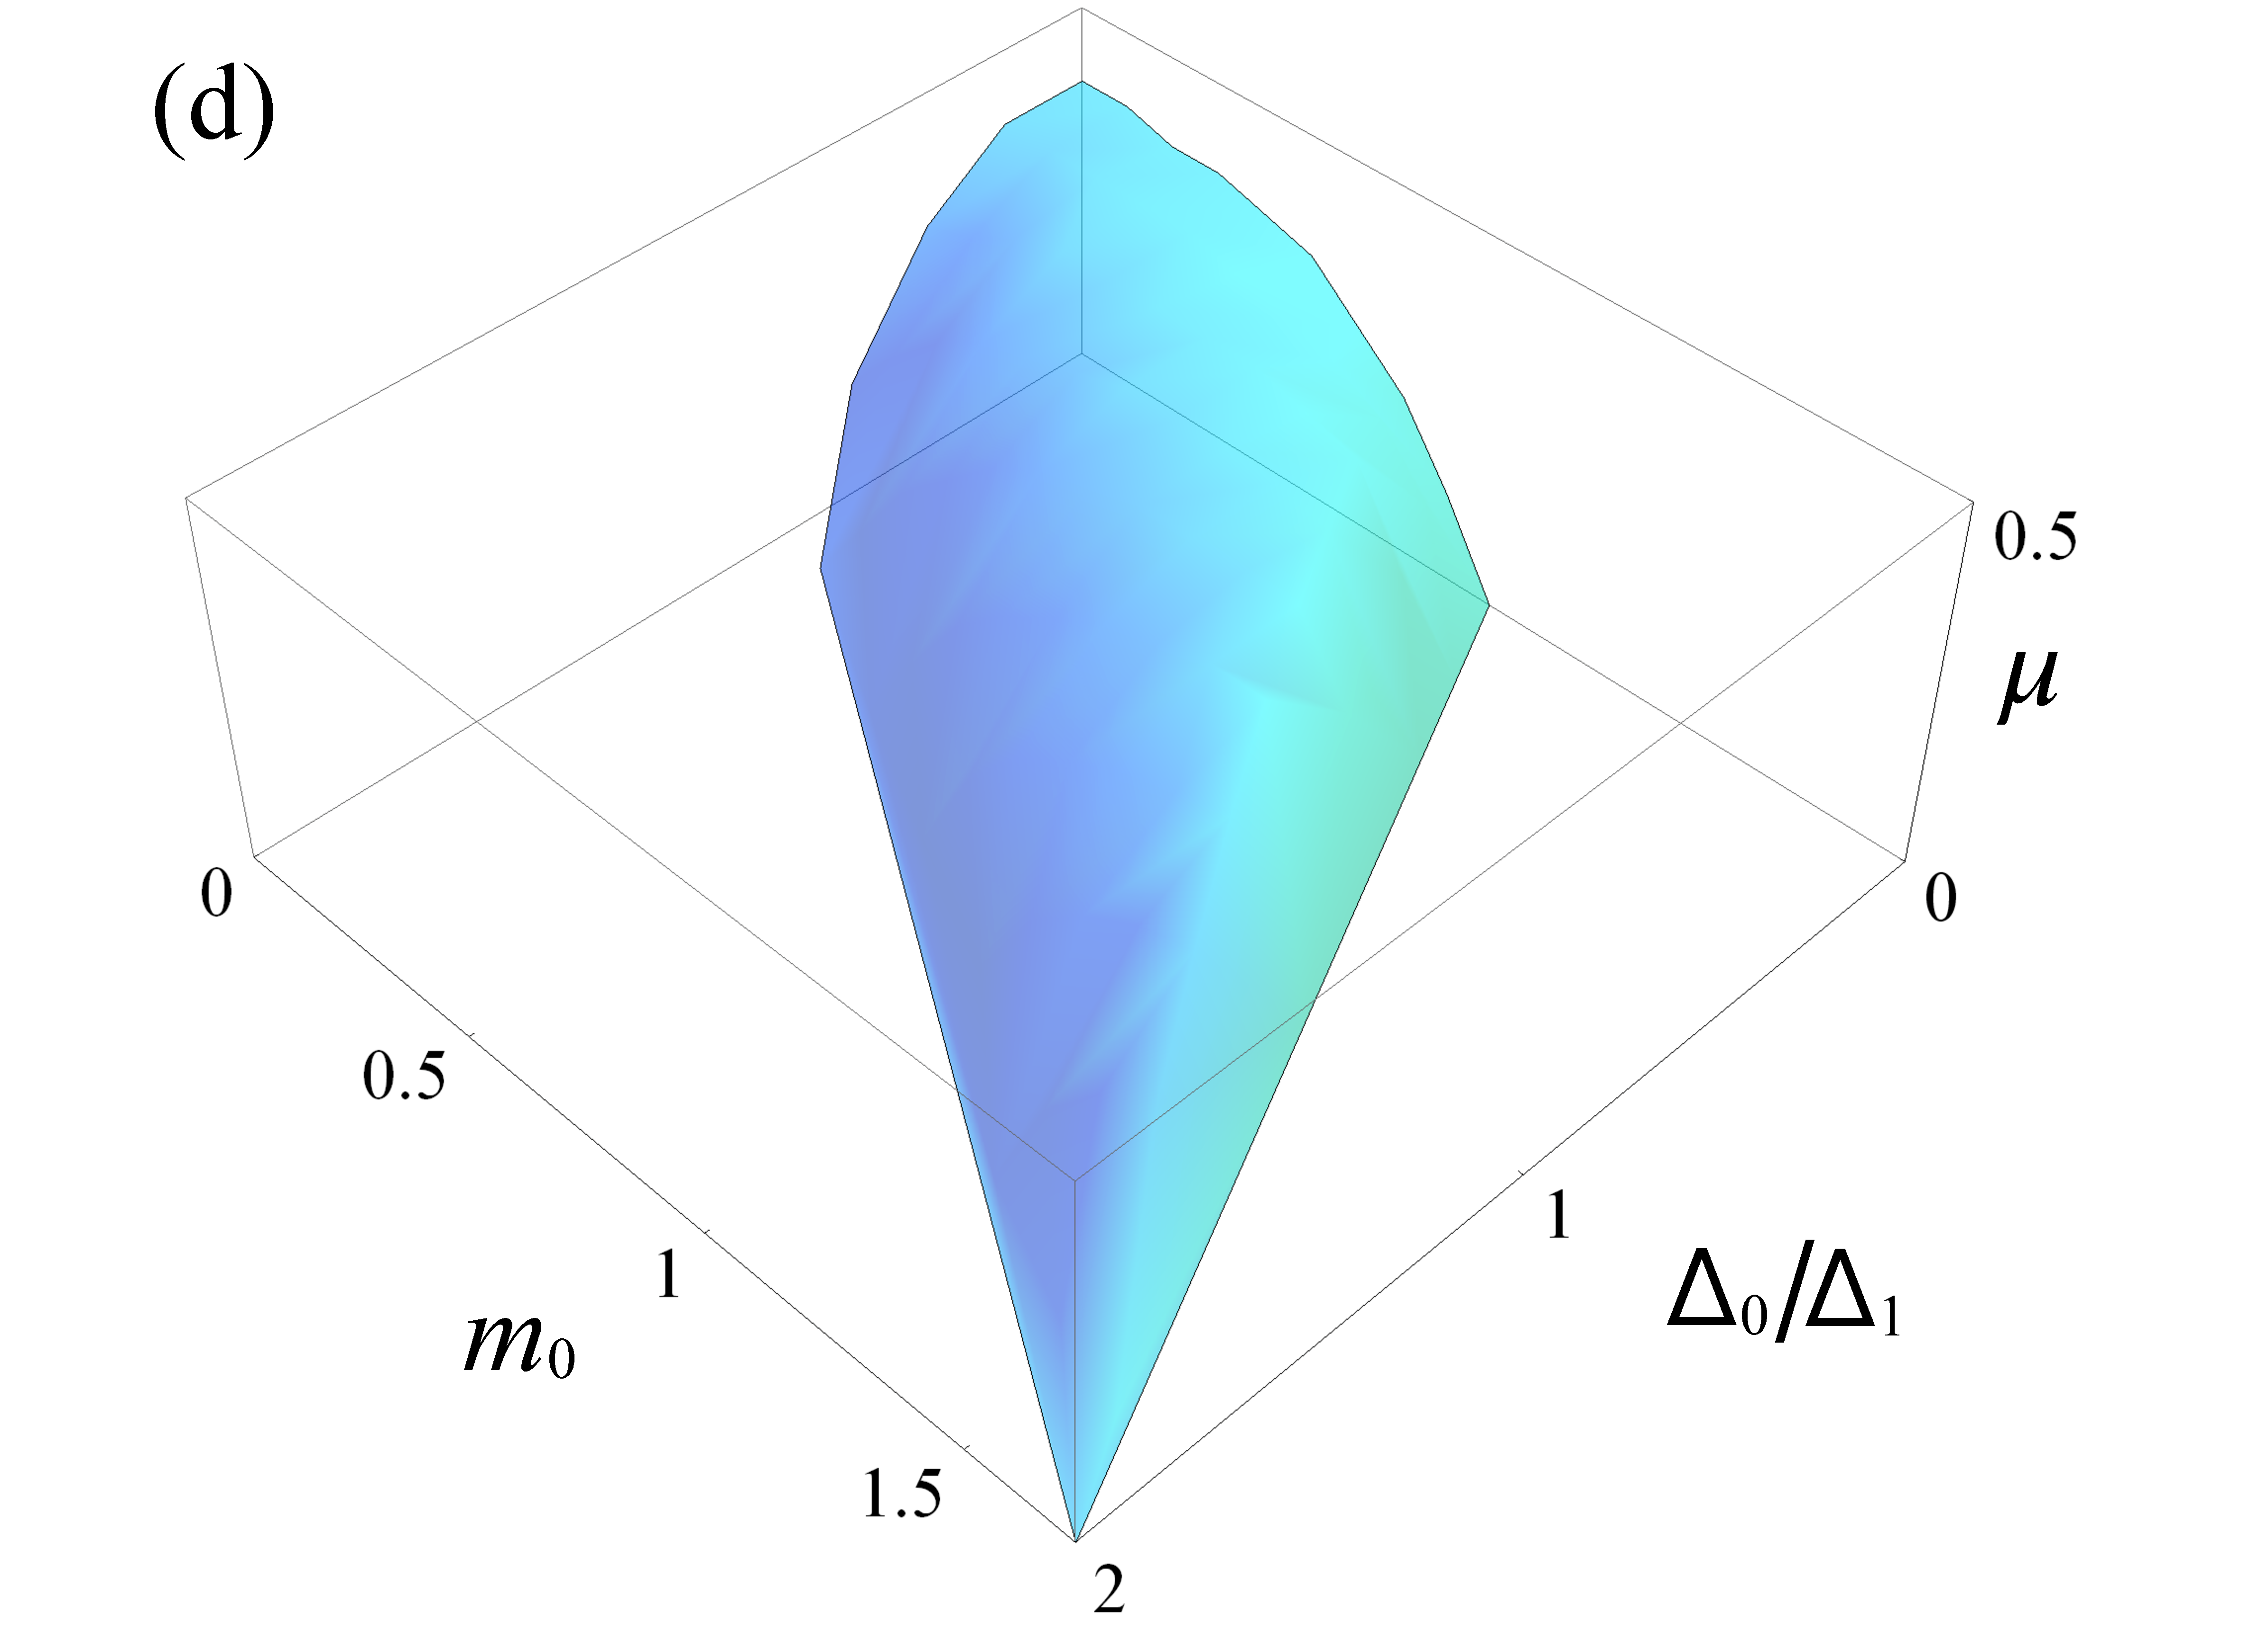
\includegraphics[scale=0.09]{pic/fig12d}
\caption{(a)能带反转环与超导配对节线环,虚线代表着$\mu=0.3$时的费米面;(b-c)零能态波函数分布,(b)中化学势$\mu=0$,(c)中化学势$\mu=0.3$;(d)($m_0,\Delta_0/\Delta_1,\mu$)相图,固定$\Delta_1=0.4$,在表面包括的范围内都可以存在MKP。}\label{fig11}
\end{figure}

\qquad 研究人员还提出了一种利用Rashba自旋轨道耦合,通过超导体的近邻效应在系统中诱导出$s_\pm$-波配对,从而实现高阶拓扑超导体的方案\cite{re27}。
\begin{equation}
\begin{aligned}
H^{\mathrm{BdG}}(\mathbf{k})&=(h^{\mathrm{TI}}(\mathbf{k})-\mu)\tau_z+\Delta(\mathbf{k})\tau_x\\
h^{\mathrm{TI}}(\mathbf{k})&=\left[2t(\cos k_x-\cos k_y)+4t_1\cos k_x\cos k_y\right]\sigma_z+2\lambda(\sin k_xs_y-\sin k_ys_x)\sigma_x\\
\Delta(\mathbf{k})&=\Delta_0+2\Delta_1(\cos k_x+\cos k_y)\label{hosc2}
\end{aligned}
\end{equation}
\qquad 在这个方案中,这个模型所描述的2D拓扑绝缘体只有一个能带反转的位置在$(\pi,0)$点,当将哈密顿量沿一个方向取开边界,另外一个方向取周期边界条件的时候,会发现不同的方向开边界其边界态出现的位置是不同,如图\ref{fig12}所示,当沿$y$方向取开边界条件,$x$方向取周期边界的时候,体系的螺旋边界态出现在$k_x=\pi$这个位置处;当沿$x$方向取开边界条件,$y$方向取周期边界的时候,体系的螺旋边界态出现在$k_y=0$这个位置处。当费米面落在体态能隙中间的时候,如果通过近邻效应诱导$s_\pm$-波配对$\Delta(\mathbf{k})=\Delta_0+2\Delta_1(\cos k_x+\cos k_y)$则边界态会被打开一个能隙,当$\Delta_0=0$时结果如图\ref{fig12}(b,d)所示。
\begin{figure}[h]
\centering
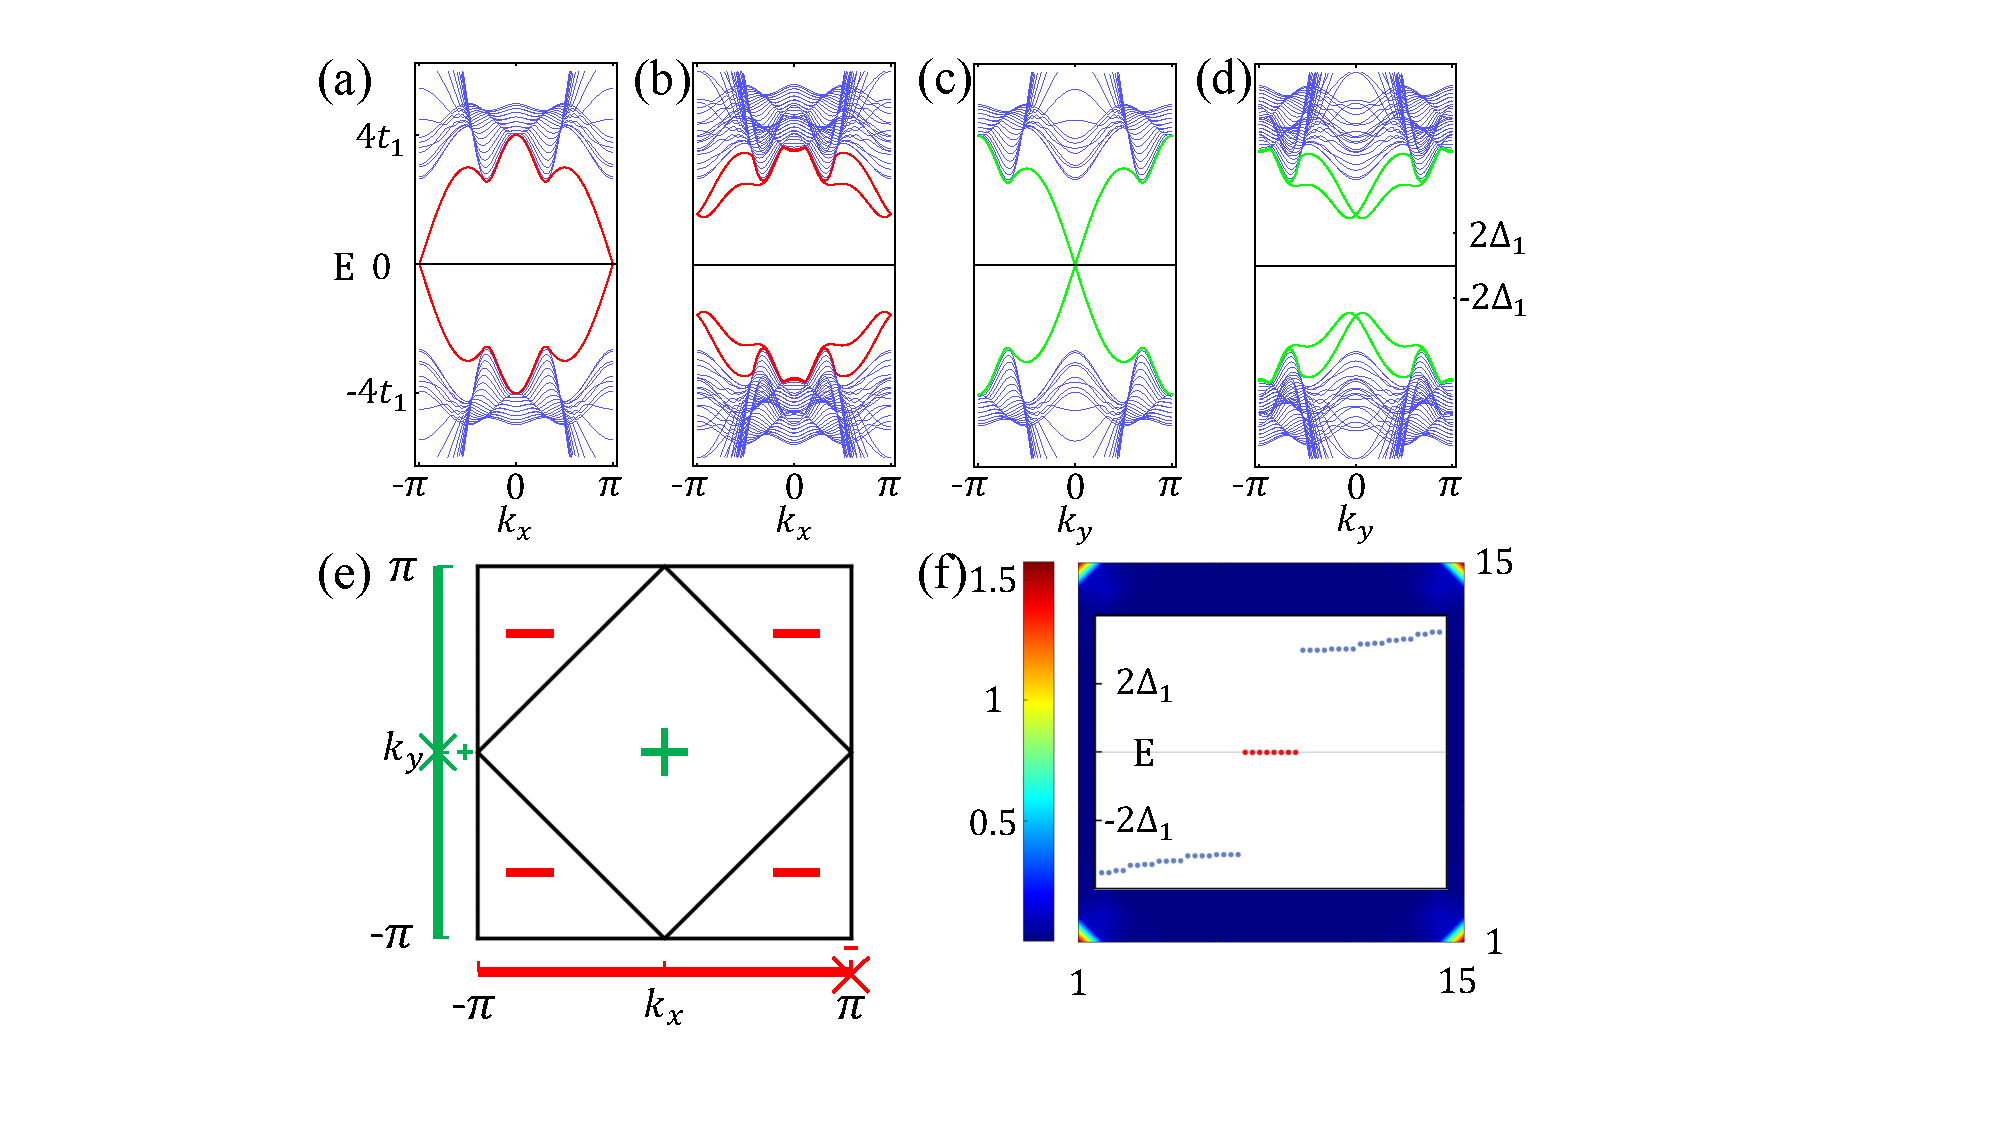
\includegraphics[scale=0.7]{pic/fig13}
\caption{(a)2D拓扑绝缘体沿($0\bar{1}$)方向圆柱体结构能带图,此时边界态出现在$k_x=\pi$;(b)能带(a)在加入$s_\pm$配对后BdG哈密顿量的能谱图;(c-d)和(a-b)相似,此时边界态出现在($\bar{1}0$)这个方向的$k_y=0$处}\label{fig12}
\end{figure}
当在一个四方结构的拓扑绝缘体中诱到$s_\pm$-波配对之后,螺旋的边界态会被打开能隙,从而在每个角落处形成MKP,结果如\ref{fig12}(f)所示。

\qquad 当化学势$\mu$比较小的时候,拐角处局域的MKP可以通过边界分析来解释,如图\ref{fig12}(e)所示,当$\Delta_0=0$的时候,在BZ中超导配对$\Delta(\mathbf{k})$是有正负变化的,在($0\bar{1}$)边界上,$k_x=\pi$处的螺旋边界态所获得的超导配对值为负,因为在$k_x=\pi$处,所有$k_y$对应的$\Delta(\mathbf{k})$都是负号;相反的在$(\bar{1}0)$边界上,$k_y=0$处的边界态所获得的超导配对负号都是正的,因为在$k_y=0$对于所有的$k_x$而言,$\Delta(\mathbf{k})$都是正号。所在这就会在相邻的两个边界处形成质量畴壁,从而在拐角处产生MKP。










